%% Author: Mohammed Hamza
%% Date:
%% Description: Generic and customizable thesis/dissertation template.
%% URL: https://github.com/Bekt/thesis-template

\documentclass[12pt,letterpaper]{report}
\usepackage[left=1.5in, right=1.0in, top=1.0in, bottom=1.0in]{geometry}

% Check if with latex or pdflatex.
\ifx\pdftexversion\undefined
  \usepackage[dvips]{graphicx}
\else
  \usepackage[pdftex]{graphicx}
\fi

\usepackage{setspace}
\usepackage{titlesec}
\usepackage{enumerate}
\usepackage{enumitem}
\usepackage{amsmath}
\usepackage{amssymb}
\usepackage{fancyvrb}
\usepackage{float}
\usepackage{hyperref}
\usepackage{svg}
\usepackage{fancyhdr} % Required for fancy page styles
\usepackage{xcolor} % Required for defining custom colors
\usepackage{listings} % Required for code listings
\usepackage{tabulary}
\usepackage{multicol}
\usepackage{times}
\usepackage{epsfig}
\usepackage{tikz}
\usepackage{amsmath}
\usepackage{amsfonts}
\usepackage{amssymb}
\usepackage{circuitikz}
% \usepackage{sagetex}
% \usepackage{graphicx}
\usetikzlibrary{shapes, arrows.meta,arrows, positioning,chains, quotes}

% variables definition
\newcommand{\memberA}{Mohammed Hamza}
\newcommand{\memberB}{Nanda kishore}
\newcommand{\memberC}{def}
\newcommand{\memberD}{xyz}
\newcommand{\memberE}{xyz}
\newcommand{\indexA}{U03NM21T043044}
\newcommand{\indexB}{150360A}
\newcommand{\indexC}{150273J}
\newcommand{\indexD}{150504V}
\newcommand{\indexE}{150504V}
\newcommand{\guideA}{Dr BPH}
\newcommand{\guideB}{Dr HMV}
%auto-ignore
\renewcommand{\vec}[1]{\mathbf{#1}}

\usepackage{caption}
\usepackage{subcaption}
\usepackage{tabularx}
\usepackage{multirow}
\usepackage{amsmath}
\usepackage{amssymb}
\usepackage{graphicx}
\usepackage{algorithm}% http://ctan.org/pkg/algorithms
%\usepackage{algpseudocode}% http://ctan.org/pkg/algorithmicx
\usepackage{algpseudocode}


\usepackage{amsthm}           
\newtheorem{thm}{Theorem}[section]
\newtheorem{lem}[thm]{Lemma}
\newtheorem{prop}[thm]{Proposition}
\newtheorem{cor}[thm]{Corollary}
\newtheorem{conj}[thm]{Conjecture}
\newtheorem{mydef}[thm]{Definition}

\renewcommand{\vec}[1]{\mathbf{#1}}

\newcommand{\Pro}{\operatorname{Pr_0}}
\newcommand{\X}{\mathbf{X}}
\newcommand{\Y}{\mathbf{Y}}
\newcommand{\Z}{\mathbf{Z}}
\newcommand{\I}{\mathbf{I}}
\newcommand{\Ninst}{N\operatorname{inst}}
\newcommand{\inst}{\texttt{inst}}
\newcommand{\x}{\vec{x}}
\newcommand{\y}{\vec{y}}
\newcommand{\z}{\vec{z}}
\newcommand{\Lstuff}{\mathcal{L}_{\operatorname{stuff}}}
\newcommand{\Lthings}{\mathcal{L}_{\operatorname{things}}}


\newcommand{\Sim}{\operatorname{Sim}}


\newcommand{\zo}{\vec{z}_1}
\newcommand{\zt}{\vec{z}_2}
\newcommand{\Cm}{\mathbb{C}^m}

\newcommand{\mylist}[1]{\begin{enumerate}#1\end{enumerate}}
  
\newcommand{\bd}[1]{\textbf{#1}}
\newcommand{\imI}{\mathrm{i}}

\newcommand{\indemp}[1]{\index{#1}\emph{#1}}

\newcommand{\minuseq}{\mathrel{{-}{=}}}
\newcommand{\pluseq}{\mathrel{{+}{=}}}
\newcommand{\coleq}{\mathrel{{:}{=}}}
\newcommand{\cl}{\operatorname{class}}

%\newcommand*\Let[2]{\State #1 $\gets$ #2}
%\algrenewcommand\alglinenumber[1]{
%    {\sf\footnotesize\addfontfeatures{Colour=888888,Numbers=Monospaced}#1}}
%\algrenewcommand\algorithmicrequire{\textbf{Precondition:}}
%\algrenewcommand\algorithmicensure{\textbf{Postcondition:}}

% Table of contents.
% \setcounter{secnumdepth}{3}
% \setcounter{tocdepth}{3}

% % Chapter title format, section format, subsection format.
% \titleformat{\chapter}
%   {\normalfont\Large\bfseries}{\thechapter}{1em}{}
% \titleformat{\section}
%   {\normalfont\Large\bfseries}{\thesection}{1em}{}
% \titleformat{\subsection}
%   {\normalfont\bfseries}{\thesubsection}{1em}{}
% 
% \titleformat{\section}[block]{\centering\Large\bfseries}{}{0pt}{} 
% \titlespacing*{\section}{0pt}{\baselineskip}{\baselineskip}
% % Chapter, section, subsection title spacings.
% \titlespacing*{\chapter}{0pt}{0ex plus 1ex minus .2ex}{2.3ex plus .2ex}
% \titlespacing*{\section} {0pt}{1ex plus 1ex minus .2ex}{1.5ex plus .2ex}
% \titlespacing*{\subsection} {0pt}{2ex plus 1ex minus .2ex}{1ex plus .2ex}

% renew counter for section numbering


% Spacing after a caption.
\setlength{\belowcaptionskip}{-15pt}

% % Spacing before a footer.
% \setlength{\skip\footins}{0.5cm}
\geometry{a4paper, margin=1in} 

\pagestyle{fancy}
\fancyhf{}
\fancyhead[L]{PLL implementation}


\pagestyle{fancy}
\fancyhf{} % Clear all header and footer fields
\fancyhead[L]{PLL}
\fancyhead[R]{\makebox[\textwidth][r]{\textbf{\nouppercase{\leftmark}}}} % Right-alig

\fancyfoot[L]{\textbf{Department of ECE}} % Left side: Department name
\fancyfoot[C]{\textbf{Jan 2025 – Apr 2025}} % Center: Semester dates
\fancyfoot[R]{\textbf{Page \thepage}} % Right side: Page number
\renewcommand{\footrulewidth}{0.4pt}
% Define a custom page style for section pages
\fancypagestyle{chapterstyle}{
  \fancyhf{} % Clear all header and footer fields
  \renewcommand{\headrulewidth}{0pt} 
  \fancyfoot[L]{\textbf{Department of ECE}} % Left side: Department name
  \fancyfoot[C]{\textbf{Jan 2025 – Apr 2025}} % Center: Semester dates
  \fancyfoot[R]{\textbf{Page \thepage}} % Right side: Page number
}

% Apply custom style to section pages
% \makeatletter
% \preto\section{\thispagestyle{sectionstyle}}
% \makeatother

% \makeatletter
% \preto\chapter{\thispagestyle{chapterstyle}}
% \makeatother

% No header on the first page of a section




% \renewcommand{\section}{
%     \clearpage % Start each section on a new page
%     \pagestyle{plain} % Remove header
%     \oldsection
%     \thispagestyle{plain} % Ensure no header on this first page
%     \pagestyle{fancy} % Resume normal header style
% } have to check thisfkdljal;dskfa;sdkl;falsd;f

\definecolor{light-gray}{gray}{0.95} % Define the light-gray color
\lstset{
  basicstyle=\ttfamily\small,
  basicstyle=\ttfamily\small,
  keywordstyle=\color{blue}\bfseries,
  stringstyle=\color{red},
  commentstyle=\color{gray},
  morekeywords={int, return, Serial, if, else}, % Add any other keywords specific to your code
  numbers=left,
  numberstyle=\tiny\color{gray},
  stepnumber=1,
  breaklines=true,
  captionpos=b,
  tabsize=2,
  showspaces=false,
  showstringspaces=false,
  showtabs=false,
  breakatwhitespace=true,
  backgroundcolor=\color{light-gray}, % Set background color
}

\begin{document}

  \onehalfspacing
  \begin{titlepage}

  \vspace{1 in}
  \begin{center}
  \newcommand*{\titlegroup}{
    \centering
    \vspace*{\baselineskip} % White space at the top of the page
	
	\rule{\textwidth}{1.6pt}\vspace*{-\baselineskip}\vspace*{2pt} % Thick horizontal line
	\rule{\textwidth}{0.4pt}\\[\baselineskip] % Thin horizontal line
	{\LARGE PLL Transistor Level Implementation} \\
	
	\rule{\textwidth}{0.4pt}\vspace*{-\baselineskip}\vspace{3.2pt} % Thin horizontal line
	\rule{\textwidth}{1.6pt}\\[\baselineskip] % Thick horizontal line
	
	\scshape % Small caps
	
	\vspace*{1\baselineskip} % Whitespace between location/year and editors
	{\large{\textsl{
				{A \\ 
					  Project Report \\ %\underline{•}
					Submitted in Partial Fulfillment of the Bangalore University\\
					for the Degree \\ 
					of\\
					\large \bf Bachelor of Technology \\
                    in\\
                    \large \bf Electronics and \\
                    \large \bf Communication Engineering 
	}}}}\\
	[5ex] \emph{by} \\[1ex]
	%Submitted by \\[\baselineskip]
  }

  \titlegroup

    % \vspace{1.5 in}
    % \vspace{50mm}
    
    % \begin{flushleft}
    % \begin{multicols}{2}
    % 	Supervisors: \\
    % 	\guideA \\
    % 	\guideB \\
    % 	\vfill\null
    % 	\columnbreak
    	
    % 	Group Members: \\
    % 	\memberA \ (\indexA) \\
    % 	\memberB \ (\indexB) \\
    % 	\memberC \ (\indexC) \\
    % 	\memberD \ (\indexD) \\
    	

    % \end{multicols}
    % \end{flushleft}
    
%	Supervisor:	 	\hfill  	Group Members: \\
%    \guideA \hfill 	\memberA  - \indexA \\
%    \guideB \hfill 	\memberB  - \indexB \\
%    					  \hfill 	 \memberC  - \indexC \\
%   						  \hfill 	 \memberD  - \indexD \\
    

  \end{center}
\end{titlepage}



  \singlespacing
  
    % Roman numeral numbering until introduction.
  \pagestyle{plain}
  \pagenumbering{arabic}
  
  % \begin{flushleft}
\large{
	Approval of the Department of Electronic \& Telecommunication Engineering \\
}
	
  \vspace{30mm}

  \normalsize
\begin{multicols}{2}
	\vfill\null
	\columnbreak
	\begin{center}

		{\makebox[7cm]{\dotfill}} \\ 
		Head, Department of Electronic \& \\
		Telecommunication Engineering
 \\
	\end{center}
\end{multicols}


  \vspace{20mm}

This is to certify that I/we have read this project and that in my/our opinion it is fully adequate, in scope and quality, as an Undergraduate Graduation Project. \\

  \vspace{10mm}
  
  Supervisor: \guideA \\
    \vspace{15mm}
  Signature:  {\makebox[7cm]{\dotfill}}
\\
    \vspace{10mm}
  Date: {\makebox[7.9cm]{\dotfill}}
\\

\end{flushleft}

  % \chapter*{Declaration}
 \addcontentsline{toc}{chapter}{Declaration}  


\begin{flushleft}
	This declaration is made on February 15, 2020. \\
	\vspace{10mm}
	\textbf{Declaration by Project Group} \\
	We declare that the dissertation entitled Project Name and the work presented in it are our own. We confirm that:
	
	\begin{itemize}[noitemsep,topsep=0pt]
		\item this work was done wholly or mainly in candidature for a B.Sc. Engineering degree at this university,
		\item where any part of this dissertation has previously been submitted for a degree or any other qualification at this university or any other institute, has been clearly stated,
		\item where we have consulted the published work of others, is always clearly attributed,
		\item where we have quoted from the work of others, the source is always given,
		\item with the exception of such quotations, this dissertation is entirely our own work,
		\item we have acknowledged all main sources of help,
		\item parts of this dissertation have been published. (see \hyperref[chapter:appendix3]{List of Publications})
	\end{itemize}

\vspace{15mm}
\begin{multicols}{2}
	{\makebox[3cm]{\dotfill}} \\ 
	Date
	\vfill\null
	\columnbreak
	
	{\makebox[7cm]{\dotfill}} \\ 
	\memberA \  (\indexA)  \\
	\vspace{12mm}
	{\makebox[7cm]{\dotfill}} \\ 
	\memberB \ (\indexB)  \\
	\vspace{12mm}
	{\makebox[7cm]{\dotfill}} \\ 
	\memberC \ (\indexC)  \\
	\vspace{12mm}
	{\makebox[7cm]{\dotfill}} \\ 
	\memberD \ (\indexD)  \\

\end{multicols}


\end{flushleft}

  % \chapter*{Declaration by Supervisor}
 \addcontentsline{toc}{chapter}{Declaration by Supervisor}

\begin{flushleft}
	I/We have supervised and accepted this dissertation for the submission of the degree. \\

	\vspace{15mm}
	
	{\makebox[6.5cm]{\dotfill}} \hfill {\makebox[5cm]{\dotfill}}  \\ 
	\guideA \hfill Date \\
	
	
	\vspace{15mm}
	
	{\makebox[6.5cm]{\dotfill}} \hfill {\makebox[5cm]{\dotfill}}  \\ 
	\guideB \hfill Date \\
	
\end{flushleft}
 
  \chapter*{Abstract}
\addcontentsline{toc}{chapter}{Abstract}

\begin{center}
	\vspace{5mm}
	\MakeUppercase{\textbf{Realtime Multi-Object Tracking and Pixelwise Segmentation}}\\
	\vspace{5mm}
	Group Members: \memberA, \memberB, \memberC, \\ \memberD \\
	\vspace{5mm}
	Supervisors: \supervisorA, \supervisorB \\
	\vspace{5mm}
\end{center}

\noindent Keywords: Vision, Perception, Detection, Tracking, Panoptic Segmentation, Siamese Network, Conditional Random Field, Recurrent Neural Network, Autonomous Systems. \\

Bleeding-edge technological pursuits ranging from self-guided robots at the research stage to mass scale industrial applications such as augmented reality, intelligent security systems and self-driving vehicles heavily rely on perception through vision. Vision based perception of the environment in autonomous systems extensively use object detection, segmentation and tracking as fundamental components. Despite the recent advancements in deep learning-based object detection on monocular images, several highly publicized accidents involving self-driving vehicles and critical failures in monitoring systems highlight the need for significant further improvement on real-time tracking systems in practice. We identify two such key areas with room for improvement and introduce two separate novel frameworks to tackle each problem. 

We observe that trackers often perform poorly in object dense situations where occlusions and crossovers are prevalent. We identify that in order to perform better in these scenarios both appearance and motion information should be incorporated. Siamese networks have recently become highly successful at appearance based single object tracking while Recurrent Neural Networks (RNNs) have started dominating motion-based tracking. Our work focuses on combining Siamese networks and RNNs to exploit both (temporally varying) appearance and motion information to build a robust framework that can also operate in real-time. We further explore heuristics-based constraints for tracking in the Bird’s Eye View Space for efficiently exploiting 3D information.

Our segmentation approach is based on one of the most overwhelming problems in current vision community that has full scale perception on the image, known as panoptic segmentation where pixel level identification of the entire image is done with both semantic and instance information thus integrating object classes (thing classes having countable instance segmentation) and back-ground classes (stuff, amorphous) in a single frame. We tackle the panoptic segmentation problem with a conditional random field (CRF) model. At each pixel, the semantic label and the instance label should be compatible and spatial and color consistency of the labeling has to be preserved (similar looking neighboring pixels should have the same semantic label and the instance label). To tackle this problem, we propose a fully differentiable model named Bipartite CRF (BCRF) which can be included as a trainable first class citizen in a deep network.

  \chapter*{Dedication}
\addcontentsline{toc}{chapter}{Dedication}

\begin{center}
	\vspace{100mm}
	To our families, friends, supervisors, and all others that supported us in this work. \\
\end{center}


  \chapter*{Acknowledgements}
\addcontentsline{toc}{chapter}{Acknowledgements}

\vspace{10mm}

\setstretch{1.5} We sincerely express our gratitude to our guide, \textbf{\guideA}, for his invaluable guidance, support, and encouragement throughout this project. We would also extend our gratitude towards Our Department's Esteemed HoD \textbf{Dr. Kiran K}. We are thankful to the Department of Electronics and Communication Engineering, UVCE, for providing us with the resources and opportunity to work on this project. Special thanks to our peers and family for their continuous motivation and assistance. We would also like to acknowledge the support of the administrative staff, whose help ensured smooth progress of our work. Additionally, we are grateful to the authors and researchers whose work has significantly contributed to our understanding and implementation. Finally, we recognize the inspiration and insights gained from discussions and feedback provided by our friends and colleagues. 


  
  \onehalfspacing
  \tableofcontents
  \addcontentsline{toc}{chapter}{Contents}
  \pagebreak
  
  \listoffigures
  \pagebreak
  
  \listoftables
  \pagebreak
  
    \chapter*{Acronyms and Abbreviations}
\addcontentsline{toc}{chapter}{Acronyms and Abbreviations}
\vspace{5mm}
\begin{tabular}{ll}
\textbf{PLL}  & Phase Locked Loop \\
\textbf{VCO}  & Voltage Controlled Oscillator \\
\textbf{PID}  & Proportional-Integral Derivative \\
\textbf{PD}   & Proportional Derivative \\
\textbf{PFD}  & Phase Frequency Detector \\
\textbf{TSMC} & Taiwan Semiconductor Manufacturing Company \\
\textbf{OTA}  & Operational Transconductance Amplifier \\
\textbf{FD}   & Frequency Divider \\
\textbf{LF}   & Loop Filter \\
\textbf{CP}   & Charge Pump \\
\end{tabular}

    \chapter*{Symbols}
\addcontentsline{toc}{chapter}{Symbols}
\vspace{5mm}
\begin{tabular}{ll}
\textbf{C}    & Capacitance \\
\textbf{R}    & Resistance \\
\textbf{W}    & Width \\
\textbf{L}    & Channel length \\
\textbf{L}    & Inductor \\
\textbf{t}    & Time \\
\boldmath$\mu$ & Electron mobility \\
\textbf{C\textsubscript{ox}} & Oxide Capacitance \\
\textbf{V\textsubscript{ov}} & Voltage Overdrive \\
\boldmath$\phi$ & Phase \\
\boldmath$\zeta$ & Damping factor \\
\boldmath$\omega$ & Frequency in radians \\
\boldmath$\tau$ & Time constant \\
\end{tabular}
  

  % Change the numbering back to normal.
  \pagestyle{plain}
  \pagenumbering{arabic}
  \setcounter{page}{1}

  \onehalfspacing
  \chapter{Introduction}
 A PLL is a feedback system that includes a VCO, phase detector, and low pass filter within its loop.Its purpose is to force the VCO to replicate and track the frequency and phase at the input when in lock. The PLL is a control system allowing one oscillator to track with another.
\begin{equation}
    \label{eq:pll_1}
    \phi_{\text{out}}(t) = \phi_{\text{in}}(t) + \text{const.}
\end{equation}
\begin{figure}[h]
    % \vspace{-0.7cm}
      \centering
      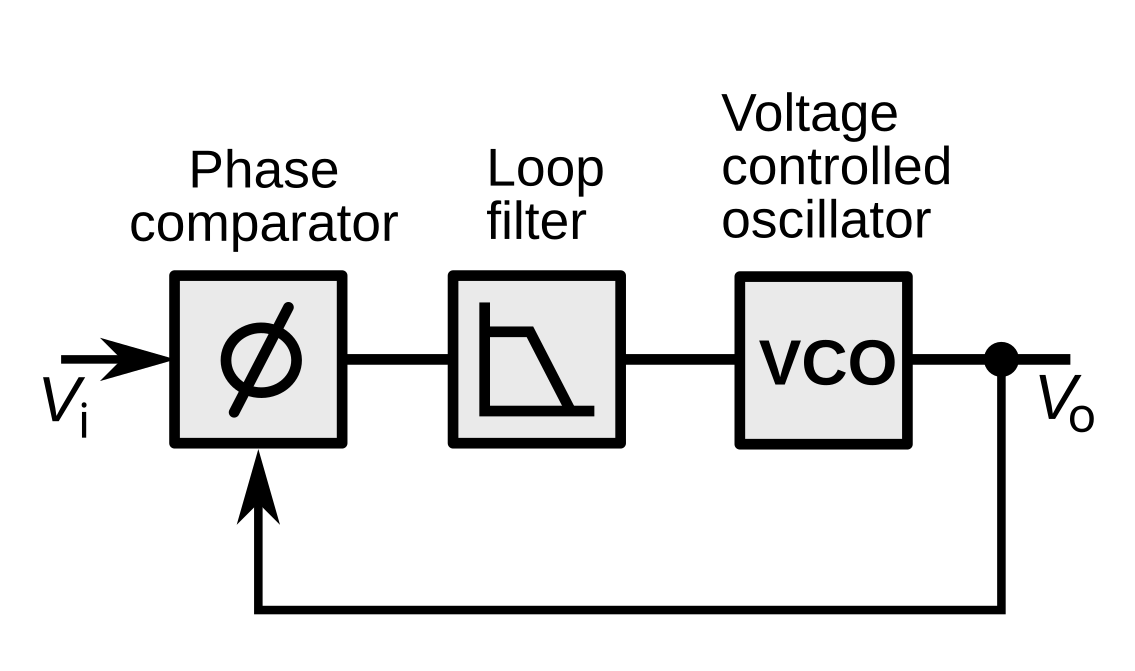
\includegraphics[width=0.5\textwidth]{figs/Phase_locked_loop.png}      \vspace{-0.3cm}
      \caption[]{ Simple analog phase locked loop}
      \label{fig:pll_1}
    % \vspace{0.5cm}
\end{figure}    
\section{Motivation}
Our team chose to work on the PLL project to gain practical knowledge about the fundamentals of phase-locked loops and their applications in modern electronics. We were particularly interested in the design and implementation of a PLL circuit at the transistor level to understand the underlying principles of PLL operation and the challenges involved in designing such circuits. We were motivated by the opportunity to work with simulation tools and techniques, such as LTspice, to analyze and optimize.

\section{Brief History and Applications of PLL}
\begin{itemize}
    \item The PLL was invented in 1932 by Harold Stephen Black, an engineer at Bell Labs.
    \item The original PLL was used in telephone systems to eliminate noise and improve the quality of voice signals.
    \item Since then, the PLL has been widely used in various applications, including:
    \begin{itemize}
        \item Clock generation: Ensuring that all components operate synchronously.
        \item Frequency synthesis: Generating a range of frequencies from a single reference frequency.
        \item Demodulation: Used in communication systems like FM radio and digital communication systems.
        \item Data recovery: Recovering clock signals from data streams for proper synchronization.
        \item Jitter reduction: Improving the performance of high-speed digital circuits.
        \item Phase alignment: Aligning the phase of multiple signals for proper timing and synchronization.
        \item Frequency modulation: Modulating signals in communication systems like FSK and PSK.
        \item Signal conditioning: Filtering and conditioning signals to improve quality and reduce noise.
        \item Clock recovery: Ensuring proper synchronization between transmitting and receiving devices.
    \end{itemize}
\end{itemize}

\section{Objective of the Project}
\begin{itemize}
    \item To design a PLL circuit at the transistor level using LTspice, with specific characteristics and specifications.
    \item Design targets:
    \begin{itemize}
        \item Reference Frequency = 20 MHz
        \item Output Frequency = 2.4 GHz
        \item Power Consumption = 2 mW
        \item Deterministic Jitter = 10 ps, pp
        \item Random Jitter = 2 ps, rms
        \item Supply Voltage = 1 V
    \end{itemize}
    \item Carry out simulations to verify the performance of the designed PLL circuit.
    \item Analyze the results and compare them with the design targets.
    \item Identify the charachteristics of the PLL circuit for example:
    \begin{itemize}
        \item Phase noise
        \item Jitter
        \item Lock time
        \item Frequency stability
        \item Power consumption
        \item Output waveform
        \item Phase margin
        \item Loop bandwidth
        \item frequecy capture range
    \end{itemize}       
    \item Document the design process, challenges faced, and lessons learned during the project.
\end{itemize}
  \chapter{Literature Review}

Phase-Locked Loops (PLLs) are critical components in modern electronic systems, widely used for frequency synthesis, clock generation, and signal synchronization. This section reviews the foundational concepts, advancements, and applications of PLLs as presented in the literature.

\section{Fundamentals of PLLs}
% The PLL is a feedback control system that synchronizes the phase of an output signal with a reference signal. Early works, such as those by Gardner \cite{gardner2005phaselock}, laid the theoretical foundation for PLL design, focusing on the mathematical modeling and stability analysis of the loop.
\section{PLL Terminologies}
A few key parameter associated with PLLs are:
\subsection{PLL bandwidth}
The PLL bandwidth is the frequency range over which the PLL can effectively track the input signal.It provides a measure by which PLL’s ability to track the input clock can be determined. It is commonly designated by the symbol \( \omega_{\text{3db}} \) It is determined by the loop filter design and affects the PLL's response time and stability.
\subsection{Natural Frequency}
The natural frequency of a PLL is the frequency at which the system oscillates when not damped. It is a critical parameter that influences the PLL's transient response and stability. The natural frequency is typically denoted by \( \omega_n \) and is determined by the loop filter and VCO characteristics.
\subsection{Damping Factor}
The damping factor is a dimensionless parameter that describes how oscillations in a system decay after a disturbance. In PLLs, it is crucial for determining the transient response and stability of the system. A damping factor of 1 indicates critical damping, while values less than 1 indicate underdamping and greater than 1 indicate overdamping.

\section{Types of PLLs}
Several types of PLLs have been developed to cater to different applications:
\begin{itemize}
    \item \textbf{Analog PLLs (APLLs):} These are the traditional PLLs that use analog components such as voltage-controlled oscillators (VCOs) and phase detectors.
    \item \textbf{Digital PLLs (DPLLs):} With advancements in digital technology, DPLLs have gained popularity due to their robustness and programmability.
    \item \textbf{All-Digital PLLs (ADPLLs):} These PLLs eliminate analog components entirely, offering better integration in digital systems.
\end{itemize}

\section{Applications of PLLs}
PLLs are employed in a wide range of applications:
\begin{itemize}
    \item \textbf{Communication Systems:} PLLs are used for carrier recovery, clock recovery, and frequency synthesis in wireless and wired communication systems.
    \item \textbf{Microprocessors:} Modern processors use PLLs for clock generation and synchronization to achieve high-speed operation.
    \item \textbf{Power Electronics:} PLLs are utilized in grid synchronization for renewable energy systems and motor control applications.
\end{itemize}

\subsection{Recent Advancements}
% Recent research has focused on improving the performance of PLLs in terms of phase noise, power consumption, and lock time. Techniques such as adaptive loop filters, machine learning-based optimization, and low-power design methodologies have been explored to enhance PLL performance \cite{recent_pll_advancements}.

\subsection{Challenges and Future Directions}
Despite significant progress, challenges remain in designing PLLs for ultra-low power applications, high-frequency operation, and integration in advanced semiconductor technologies. Future research is expected to address these challenges by leveraging emerging technologies such as quantum computing and advanced materials.

% \bibliographystyle{IEEEtran}
% \bibliography{references} 
  \chapter{Methodology/Design/Implementation}
\label{chapter:method}
\section{Phase Locked Loop System Overview}
\label{sec:pll_overview}
A Phase-Locked Loop (PLL) is a negative feedback control system circuit. As the name implies, the purpose of a PLL is to generate a signal whose phase matches that of a reference signal. This is achieved through multiple iterations of comparing the reference and feedback signals (ref fig:\ref{fig:pll_1}). The overall goal of the PLL is to align the phases of the reference and feedback signals—this is referred to as the lock mode. Once locked, the PLL continues to compare the two signals, but since they are in lock mode, the PLL output remains constant. \\
\textbf{A basic PLL consists of four main components:}
\begin{enumerate}
	\item Phase Detector or Phase Frequency Detector (PD or PFD)
	\item Charge Pump (CP)
	\item Low Pass Filter (LPF)
	\item Voltage-Controlled Oscillator (VCO)
\end{enumerate}
The Phase Frequency Detector (PFD) measures the phase difference between the reference and feedback signals. If a phase difference exists, it generates synchronized “up” or “down” signals to the charge pump and low pass filter. If the error signal from the PFD is an “up” signal, the charge pump adds charge to the LPF capacitor, increasing the control voltage, \( V_{\text{cntrl}} \). Conversely, if the error signal is a “down” signal, the charge pump removes charge from the LPF capacitor, decreasing \( V_{\text{cntrl}} \).\tikzstyle{block} = [draw, rectangle]
\tikzstyle{input} = [coordinate]
\tikzstyle{output} = [coordinate]
\tikzstyle{pinstyle} = [pin edge={to-,thin,black}]
\begin{figure}[h]
    \centering
    \begin{tikzpicture}[
      block/.style={draw, thick, minimum width=3cm, minimum height=2.5cm, align=center},
      line/.style={-Stealth, thick},
      node distance=1.5cm and 1.5cm
    ]
    
    % Blocks
    \node[input,name=inputref] (input) {fref};
    \node[block, right=2cm of input] (pd) {PD};
    \node[block, right of=pd] (cp) {CP};
    \node[block, right of=cp] (vco) {VCO};
    \node[block, below of=cp , node distance=1cm] (lpf) {LPF};
    
% Signals
\coordinate[left=1.5cm of pd] (inputref);
\coordinate[below=0cm of inputref] (inputfb);
\coordinate[right=1.5cm of vco] (output);
    
    % Connections
    % \draw [->] (inputref) -- node {$fref$} (pd);
    % \draw[--] (inputref) node[left] {$f_{ref}$} -- (pd);
    % \draw[--] (inputfb) node[left] {$f_{fb}$} -- (pd);
    \draw[line] ( inputref) -- node[above] {$f\_ref$} (pd);
    \draw[line] (inputfb) -- node[above] {$f\_fb$} ([yshift=2cm]pd);
    % \draw[--] (pd) -- (cp);
    % \draw[line] (cp) -- node[above] {$V_{cntrl}$} (vco);
    % \draw[line] (cp) |- (lpf);
    % \draw[line] (lpf) -| (vco);
    
    % \draw[line] (vco) -- node[above] {$f_{out}$} (output);
    % \draw[line] (output) |- ++(0,-2) -| (inputfb);
    
    \end{tikzpicture}
    \caption{PLL Block Diagram}
\end{figure}\\
The control voltage \( V_{\text{cntrl}} \) serves as the input to the VCO. The LPF is essential for allowing only DC signals into the VCO and for storing the charge from the CP. The VCO adjusts the feedback signal's frequency based on the error generated by the PFD. If the PFD generates an “up” signal, the VCO speeds up the feedback signal. Conversely, if a “down” signal is generated, the VCO slows it down. The output of the VCO is then fed back to the PFD to recalculate the phase difference, thereby creating a closed-loop frequency control system.

\subsection{Phase Detector}
A phase detector is a circuit that detects the difference in phase between its two input
signals. An example of a basic phase detector is the XOR gate. It produces error pulses on both
falling and rising edges.

\begin{figure}[!h]
\centering
\resizebox{0.3\textwidth}{!}{%
\begin{circuitikz}
\tikzstyle{every node}=[font=\huge]
% \draw (11.75,11.25) to[short] (12.25,11.25);
% \draw (11.75,10.75) to[short] (12.25,10.75);
\draw (12.25,11.25) node[ieeestd xor port, anchor=in 1, scale=1](port){} (port.out) to[short] (14.25,11);
\node [font=\LARGE] at (11.25,11.5) {$\phi_{\text{ref}}$};
\node [font=\LARGE] at (11.25,10.75) {$\phi_{\text{vco}}$};
\end{circuitikz}
}%
\label{fig:xor_gate}
\caption{}
\end{figure}
\subsubsection{Phase Frequency Detector}
A phase frequency detector (PFD) is a circuit that detects the difference in phase and frequency between its two input signals. The PFD is a more advanced version of the basic phase detector. It can detect both phase and frequency differences, making it more suitable for applications where the input signals may have different frequencies. The PFD generates an error signal that is proportional to the phase and frequency difference between the two input signals. This error signal is then used to control the charge pump and low pass filter in the PLL.
\begin{figure}[h]
    \centering
    \resizebox{0.8\textwidth}{!}{%
    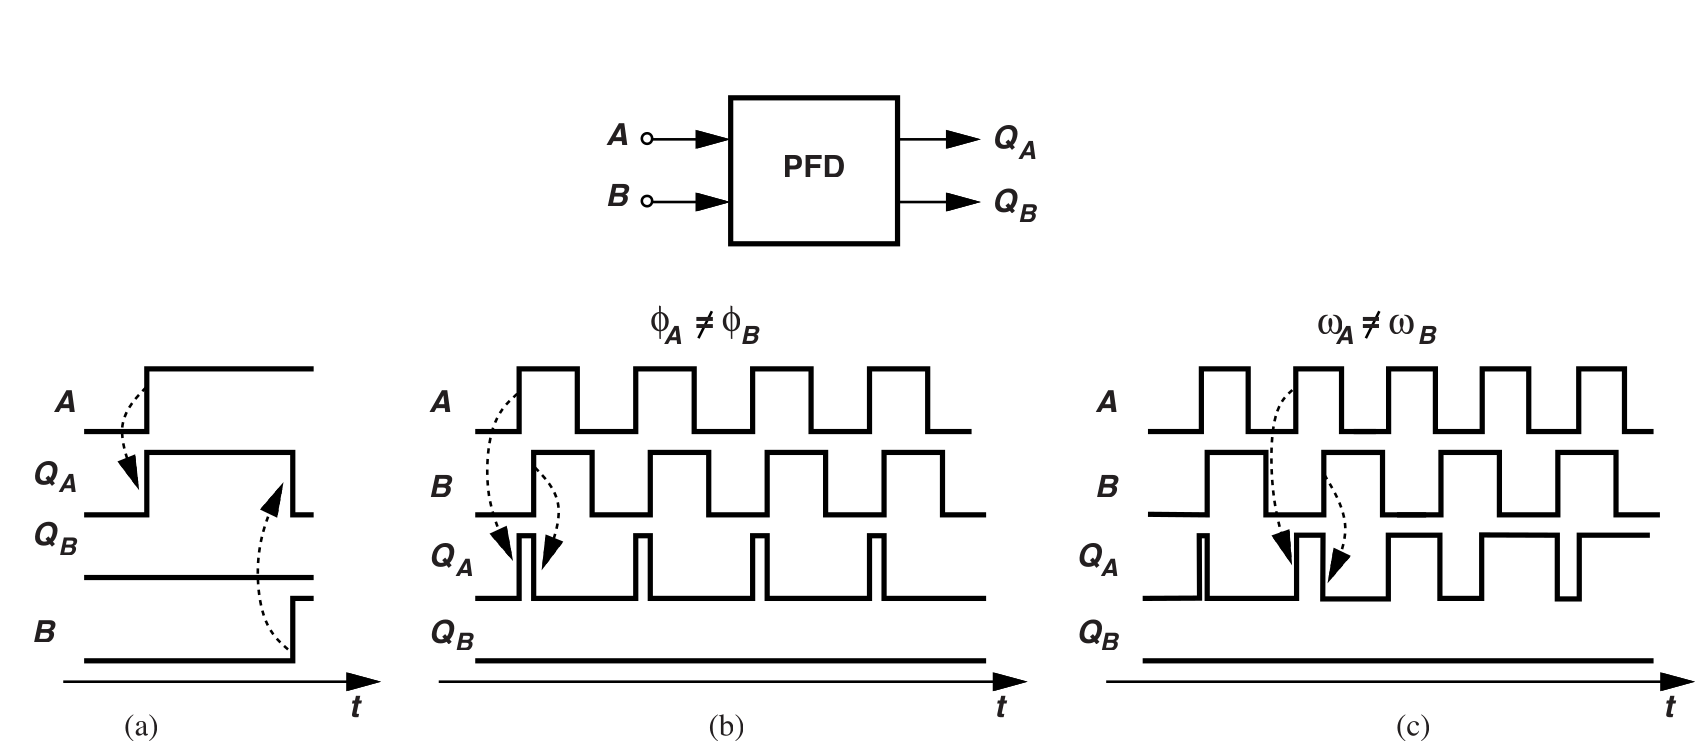
\includegraphics{figs/pfd_block.png}
    }%
    \caption{(a) Conceptual PFD operation, (b) case of input phase difference, and (c) case of input frequency difference}
    \label{fig:pfd_block}
\end{figure}
\subsection{Nanda biceps Pump}
The charge pump is a circuit that converts the error signal from the phase detector into a control voltage for the VCO. The charge pump consists of two switches and a capacitor. The switches are controlled by the error signal from the phase detector. When the error signal is high, the switch connects the capacitor to the power supply, charging it. When the error signal is low, the switch connects the capacitor to ground, discharging it. The control voltage for the VCO is taken from the capacitor.
\begin{figure}[!ht]
    \centering
    \resizebox{0.2\textwidth}{!}{%
    \begin{circuitikz}
    \tikzstyle{every node}=[font=\large]
    
    
    \draw [ line width=0.6pt](10.75,16) to[american current source,l={ \large Icp}] (10.75,14);
    \draw [ line width=0.6pt](10.75,11.75) to[american current source,l={ \large Icp}] (10.75,9.5);
    \draw [line width=0.6pt](10.75,11.75) to[normal open switch] (10.75,12.5);
    \draw [line width=0.6pt](10.75,12.5) to[normal open switch] (10.75,14);
    \draw [line width=0.6pt](10.75,9.75) to (10.75,9.5) node[ground]{};
    \draw [ line width=0.6pt](10.25,16) to[short] (11.25,16);
    \draw [ line width=0.6pt](10.75,12.75) to[short, -o] (12,12.75) ;
    \draw [ line width=0.6pt](10.75,12) to[short, -o] (9.25,12) ;
    \draw [ line width=0.6pt](10.75,13.25) to[short, -o] (9.25,13.25) ;
    \node [font=\large] at (12.5,13) {Iout};
    \node [font=\large] at (8.25,13.25) {Up};
    \node [font=\large] at (8.5,12) {Down};
    \end{circuitikz}
    }%
    
    \label{fig:my_label}
\end{figure}
\subsection{Low Pass Filter}
The low pass filter is a circuit that removes high frequency noise from the control voltage generated by the charge pump. The low pass filter consists of a resistor and a capacitor. The resistor limits the current flowing into the capacitor, while the capacitor stores the charge. The output of the low pass filter is a smooth control voltage that is fed to the VCO.
% \input{figs/lpf.tex}
\subsection{Voltage Controlled Oscillator}
The voltage controlled oscillator (VCO) is a circuit that generates an output signal whose frequency is proportional to the control voltage. The VCO consists of a transistor and a capacitor. The transistor is biased by the control voltage, which determines its operating frequency. The output of the VCO is fed back to the phase detector to complete the PLL loop.
\begin{equation}
	\label{eq:vco_char}
	f_{out} = K_{vco} * V_{in} + f_{min}
\end{equation}
\begin{figure}[h]
    \begin{subfigure}[][][1]{0.5\textwidth}
        \centering
    \resizebox{1\textwidth}{!}{%
    \begin{circuitikz}
    \tikzstyle{every node}=[font=\Large]
    
    
    \draw [ line width=0.6pt ] (8,16.5) rectangle  node {\Large VCO} (13.25,13.25);
    \draw [->, >=Stealth] (6.75,15) -- (8,15);
    \draw [->, >=Stealth] (13.25,15) -- (14.75,15);
    \node [font=\Large] at (5.5,15) {$V_{Cntrl}(V_{C})$};
    \node [font=\Large] at (15.3,15) {$f_{out}$};
    \end{circuitikz}
    }%
    \end{subfigure}
    \begin{subfigure}[][][1]{0.5\textwidth}
        \centering
            \centering
            \begin{tikzpicture}[
                axis/.style={->, thick},
                dashedline/.style={dashed, thick},
                solidline/.style={thick},
                font=\small,
                scale=1.2
            ]
            
            % Axes
            \draw[axis] (0,0) -- (6,0) node[right] {$V_C$};
            \draw[axis] (0,0) -- (0,5) node[above] {$f$};
            
            % Coordinates
            \coordinate (Vcmin) at (1,0);
            \coordinate (Vcnom) at (3,0);
            \coordinate (Vcmax) at (5,0);
            
            \coordinate (fcmin) at (0,1);
            \coordinate (fcnom) at (0,3);
            \coordinate (fcmax) at (0,4.5);
            
            \coordinate (p1) at (1,1);
            \coordinate (p2) at (3,3);
            \coordinate (p3) at (5,4.5);
            
            % Vertical dashed lines
            \draw[dashedline] (Vcmin) -- (p1);
            \draw[dashedline] (Vcnom) -- (p2);
            \draw[dashedline] (Vcmax) -- (p3);
            
            % Horizontal dashed lines
            \draw[dashedline] (fcmin) -- (p1);
            \draw[dashedline] (fcnom) -- (p2);
            \draw[dashedline] (fcmax) -- (p3);
            
            % VCO Line
            \draw[solidline] (p1) -- (p3);
            
            % Labels
            \node[below] at (Vcmin) {$V_{C(\min)}$};
            \node[below] at (Vcnom) {$V_{C(\text{nom})}$};
            \node[below] at (Vcmax) {$V_{C(\max)}$};
            
            \node[left] at (fcmin) {$f_{o(\min)}$};
            \node[left] at (fcnom) {$f_{o(\text{nom})}$};
            \node[left] at (fcmax) {$f_{o(\max)}$};
            
            \end{tikzpicture}
    \end{subfigure}            
    \caption{VCO Block Diagram and Characteristics}
    \label{fig:vco_block}
    % \vspace{-0.5cm}
\end{figure}
The VCO transfer function can be given as
\begin{equation}
	\label{eq:vco_tf}
	H_{vco}(s) = \frac{\phi_{o}(s)}{v_{o}(s)} = \frac{K_{vco}}{S}
\end{equation}
The gain of the voltage-controlled oscillator is simply the slope of the curves given in Fig.\ref{fig:vco_block}. This gain can be written as
\begin{equation}
	\label{eq:vco_gain}
	K_{vco} = 2\pi  * \frac{f_{max} - f_{min}}{V_{max} - V_{min}}(radians/s * V)
\end{equation}
Kvco is an important factor it Determines the PLL settling time.
There are different types of VCO like : Cross Coupled LC VCO, Current Starved VCO, Colpitts Oscillator. For this project, Current Starved VCO is used.
\subsection{Frequency Divider}
The frequency divider is a circuit that divides the frequency of the output signal from the VCO by a fixed integer value. The frequency divider is used to reduce the frequency of the output signal to match the frequency of the reference signal. The frequency divider can be implemented using a flip-flop or a counter. The output of the frequency divider is fed back to the phase detector to complete the PLL loop.
\section{Design of the PLL blocks}
\subsection{Phase and Frequency Detector Design}
\subsection{Charge Pump Design}
\subsection{Low Pass Filter Design}
\subsection{Voltage Controlled Oscillator Design}
In this section the Design of VCO has been shown.We have choosen current starved VCO for our design. The current starved VCO is a type of voltage-controlled oscillator (VCO) that uses a current source to control the frequency of oscillation. The basic idea behind the current starved VCO is to use a current source to control the charging and discharging of a capacitor, which in turn determines the frequency of oscillation. The current starved VCO is widely used in PLL circuits because it is simple to implement and can be easily integrated into CMOS technology.
The VCO should be Linear in a particular Operating region. The PLL built in this project will be of of the application 1GHz


% 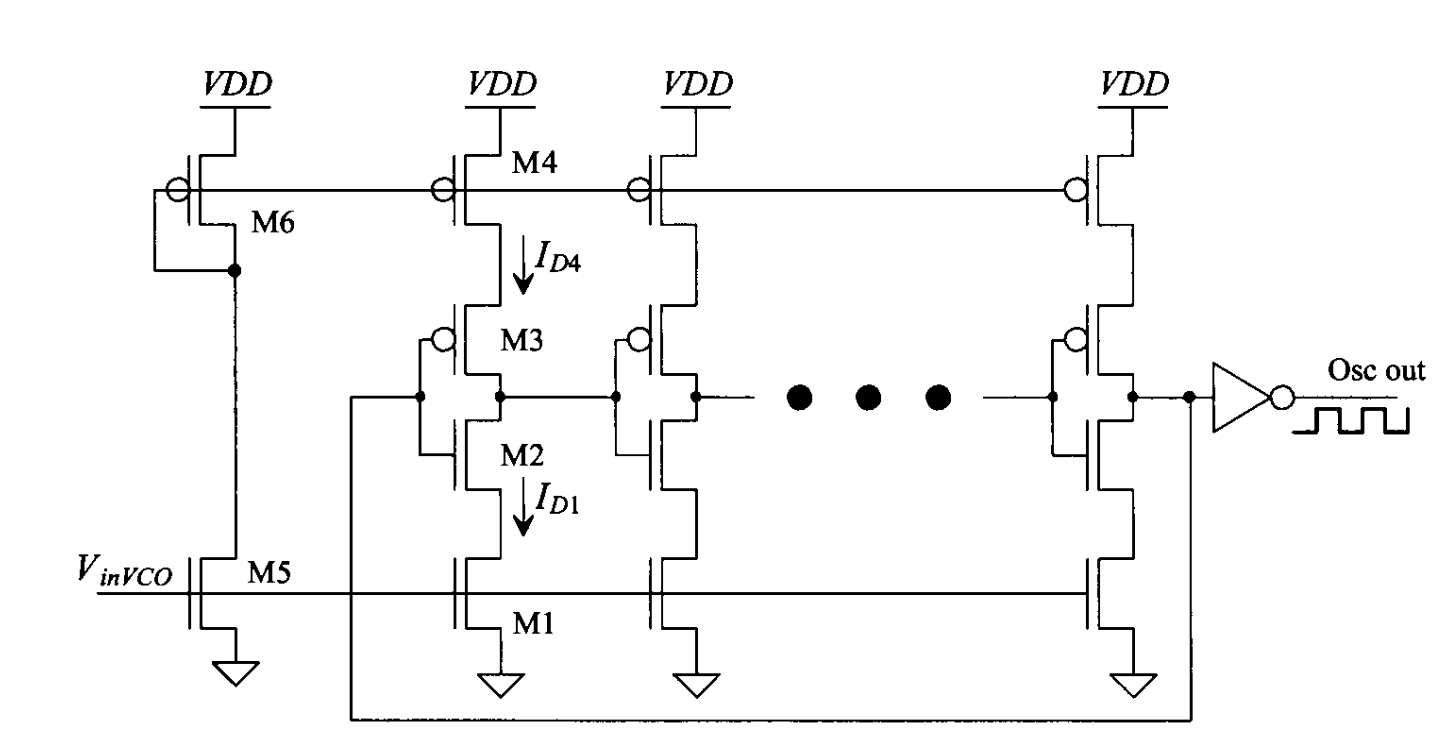
\includegraphics[0.6\textwidth]{figs/cs_vco_design.png}
\begin{figure}[h]
	\centering
	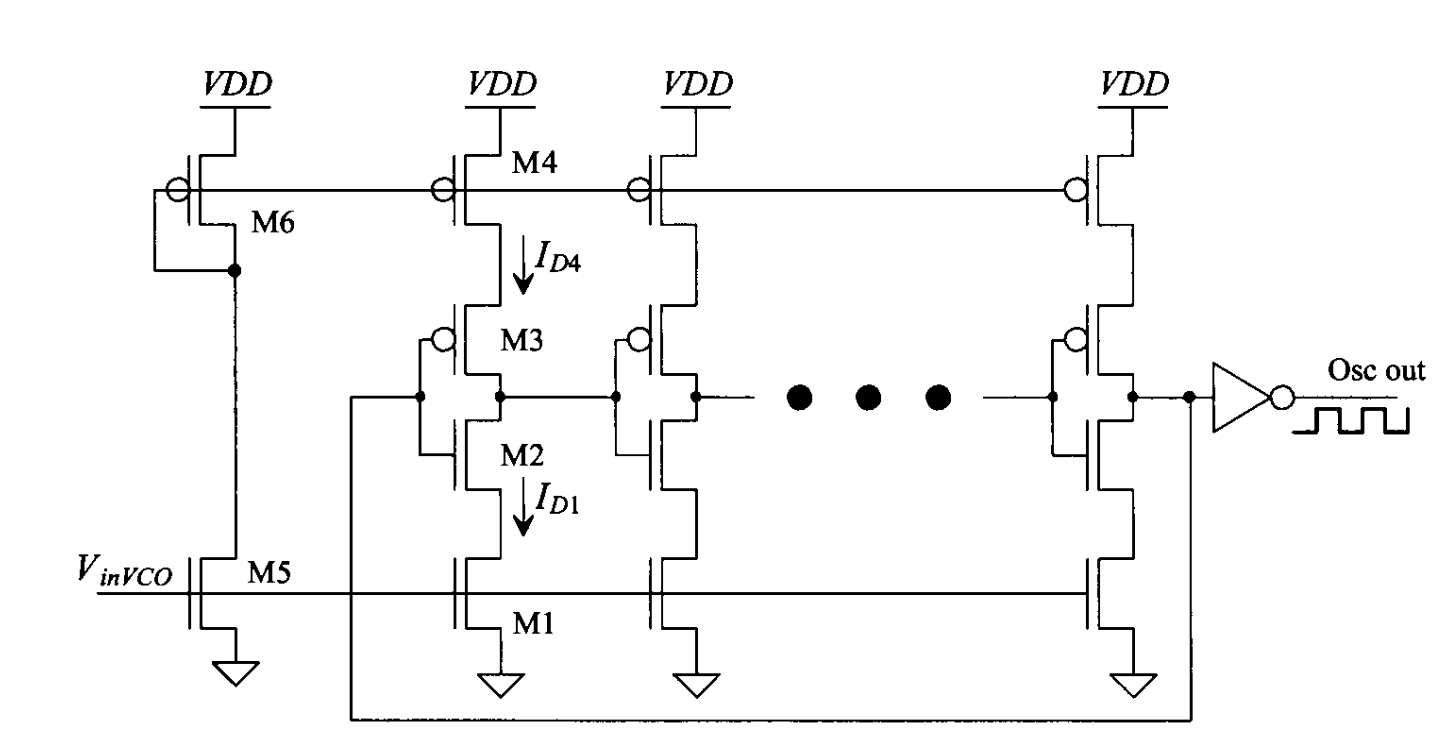
\includegraphics[width=0.5\textwidth]{figs/cs_vco_design.png}
	% \vspace{-0.3cm}
	\caption{Current Starved VCO Design}
	\label{fig:cs_vco_design}
	\vspace{0.5cm}
\end{figure}
\begin{figure}[h]
	\centering
	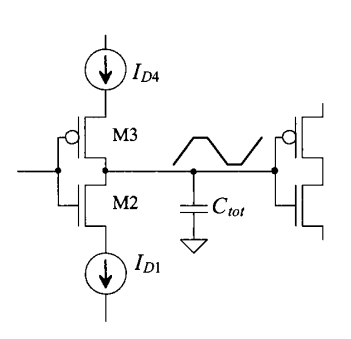
\includegraphics[width=0.5\textwidth]{figs/vco_simplified.png}
	% \vspace{-0.3cm}
	\caption{Simplified view of a single stage of the current-starved VCO}
	\label{fig:vco_simplified}
\end{figure}

To determine the design equations for use with the current-starved VCO, consider
the simplified schematic of one stage of the VCO fig \ref{fig:vco_simplified}. The total
capacitance on the drains of M2 and M3 is given by
\begin{equation}
	C_{\text{total}} = C_{\text{out}} + C_{\text{in}} = 
\underbrace{C'_{\text{ox}}(W_p L_p + W_n L_n)}_{\text{C\textsubscript{out}}} + 
\underbrace{\frac{3}{2} C'_{\text{ox}}(W_p L_p + W_n L_n)}_{\text{C\textsubscript{in}}}
\end{equation}
which is simply the output and input capacitances of the inverter. This equation can be written in a more useful form as
\begin{equation}
C_{\text{tot}} = \frac{5}{2} C'_{\text{ox}} (W_p L_p + W_n L_n)
\tag{19.19}
\end{equation}

\noindent The time it takes to charge $C_{\text{total}}$ from zero to $V_{SP}$ with the constant-current $I_{D4}$ is given by
\begin{equation}
t_1 = C_{\text{tot}} \cdot \frac{V_{SP}}{I_{D4}}
\tag{19.20}
\end{equation}

\noindent while the time it takes to discharge $C_{\text{total}}$ from $V_{DD}$ to $V_{SP}$ is given by
\begin{equation}
t_2 = C_{\text{tot}} \cdot \frac{V_{DD} - V_{SP}}{I_{D1}}
\tag{19.21}
\end{equation}

If we set $I_{D4} = I_{D1} = I_D$ (which we will label $I_{\text{Dcenter}}$ when $V_{\text{inVCO}} = V_{DD}/2$), then the sum of $t_1$ and $t_2$ is simply
\begin{equation}
t_1 + t_2 = \frac{C_{\text{tot}} \cdot V_{DD}}{I_D}
\tag{19.22}
\end{equation}

The oscillation frequency of the current-starved VCO for $N$ (an odd number $\geq 5$) of stages is
\begin{equation}
f_{\text{osc}} = \frac{1}{N(t_1 + t_2)} = \frac{I_D}{N \cdot C_{\text{tot}} \cdot V_{DD}}
\tag{19.23}
\end{equation}

which is $f_{\text{center}}(@ V_{\text{inVCO}} = V_{DD}/2 \text{ and } I_D = I_{\text{Dcenter}})$

firstly we have designed the Inverter stages and sized them accordingly and cascaded them to our required and connected a current Mirror to all the stages as in the Fig \ref{fig:vco_circuit}. The current mirror is used to control the current flowing through the inverter stages and thus control the frequency of oscillation. The output of the VCO is taken from the output of the last inverter stage. The VCO is designed to operate at a frequency of 1 GHz.
\begin{figure}[h]
	\centering
	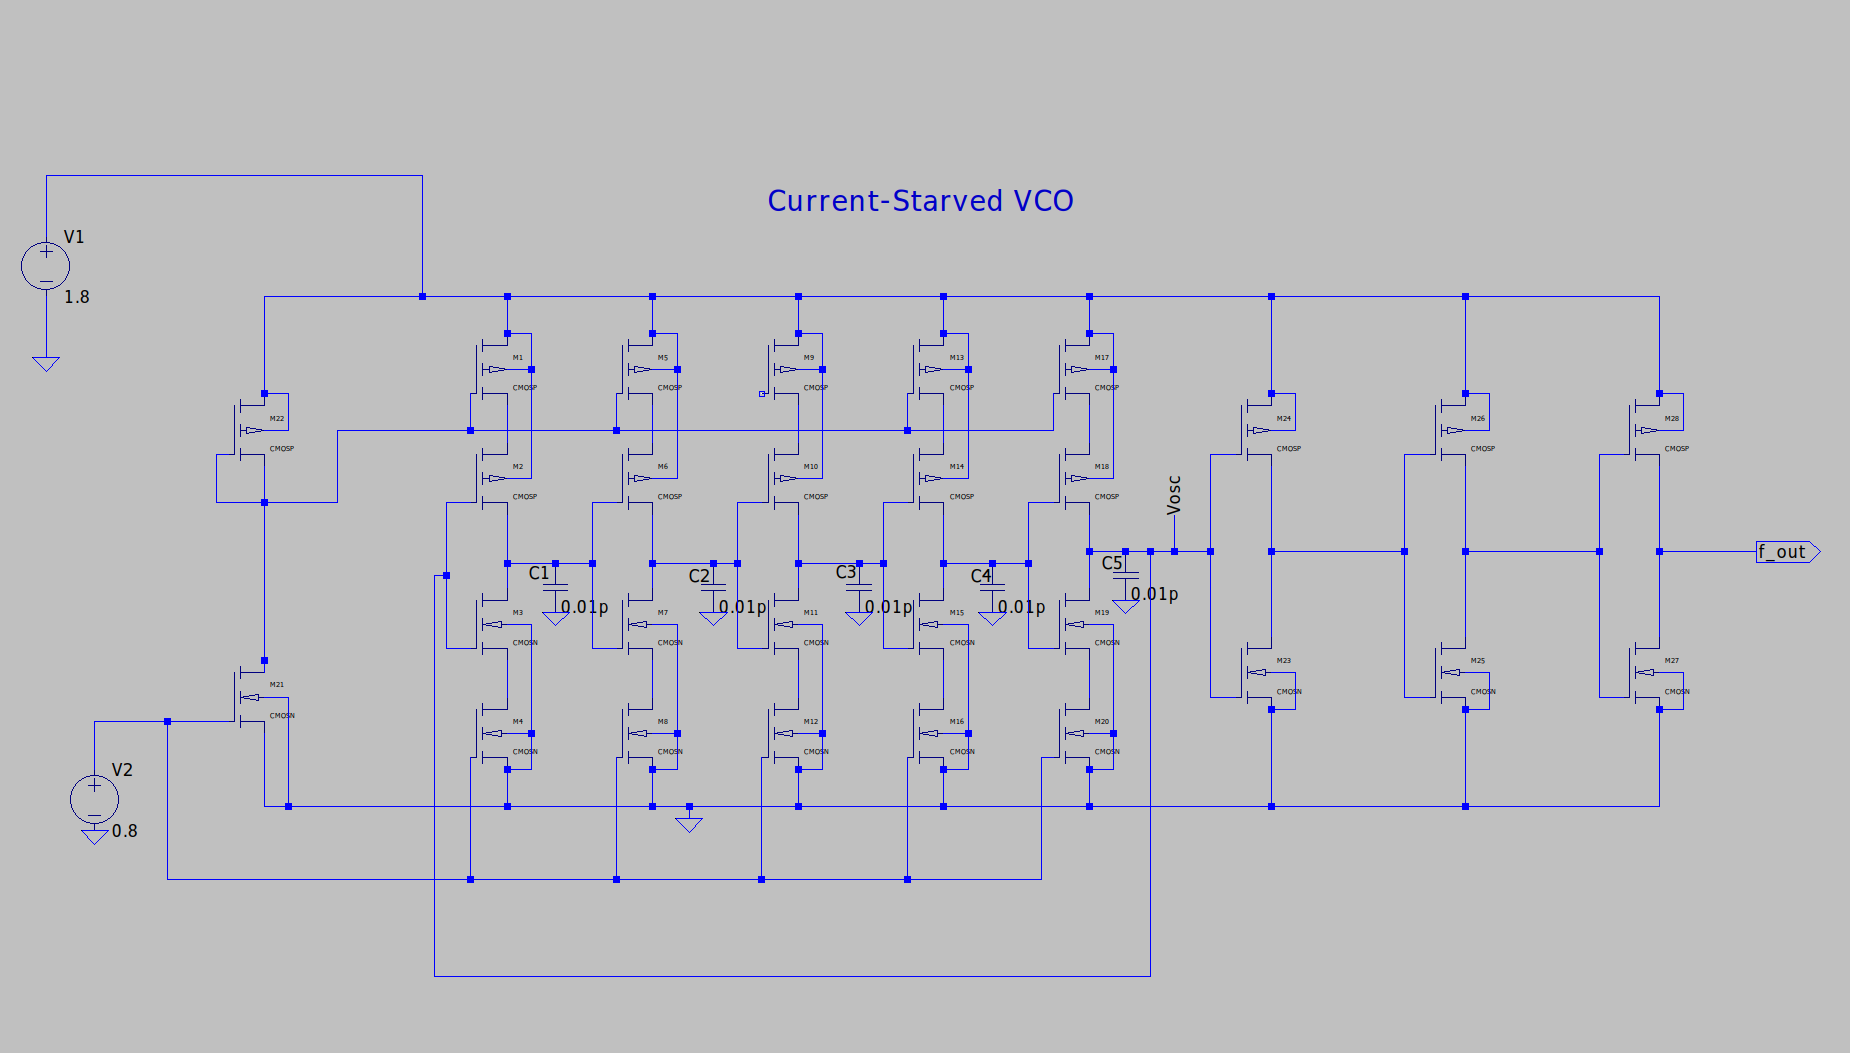
\includegraphics[width=0.9\textwidth]{figs/vco_c.png}
	% \vspace{-0.3cm}
	\caption{Current Starved VCO Circuit}
	\label{fig:vco_circuit}
	\vspace{0.5cm}
\end{figure}\\
The VCO ouput is not inherently a square wave (refer fig:\ref{fig:vco_op_c}) due to non-Ideal charachteristic of inverter here the ouput of the VCO is a irregular triangular wave. The output of the VCO is fed to a buffer and an inverter to convert the  of triangular wave to a square wave.
\begin{figure}
	\centering
	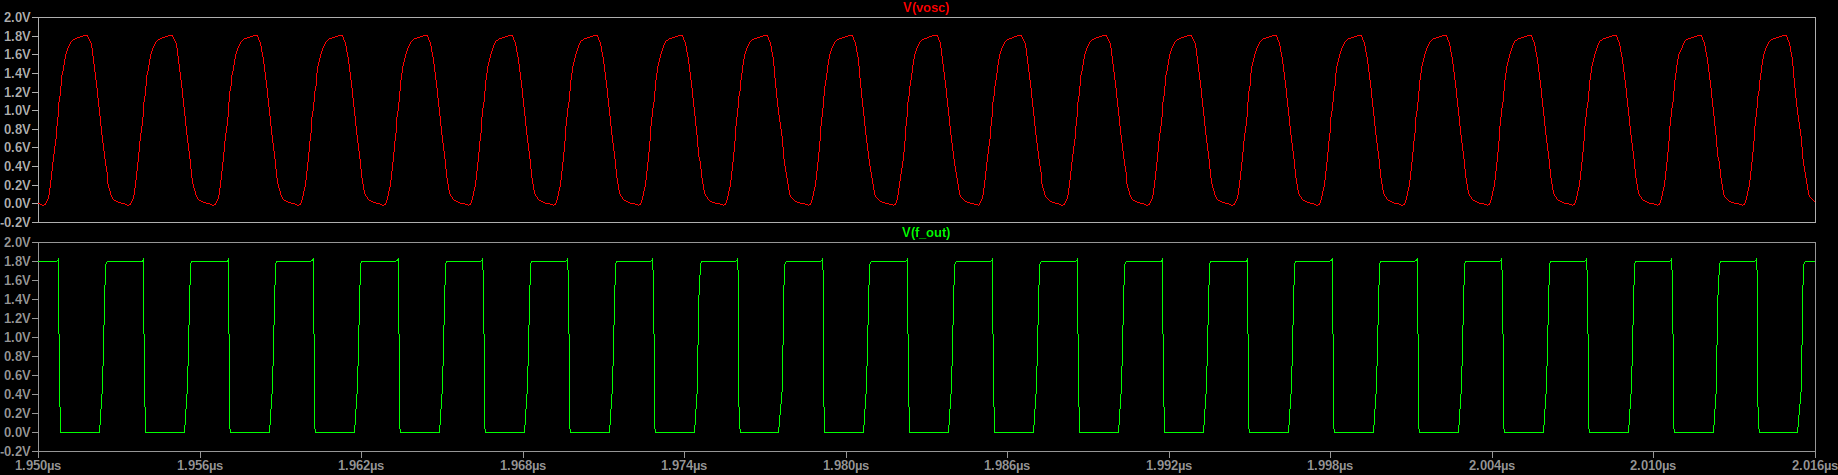
\includegraphics[width=0.9\textwidth]{figs/vco_op_both.png}
	% \vspace{-0.3cm}
	\caption{VCO output waveform before and after buffer+inverter}
	\label{fig:vco_op_c}
	\vspace{0.5cm}
\end{figure}
In Figure \ref{fig:vco_sim}, the Transient analysis of circuit in Figure \ref{fig:vco_circuit} is shown.
\begin{figure}[H]
	\centering
	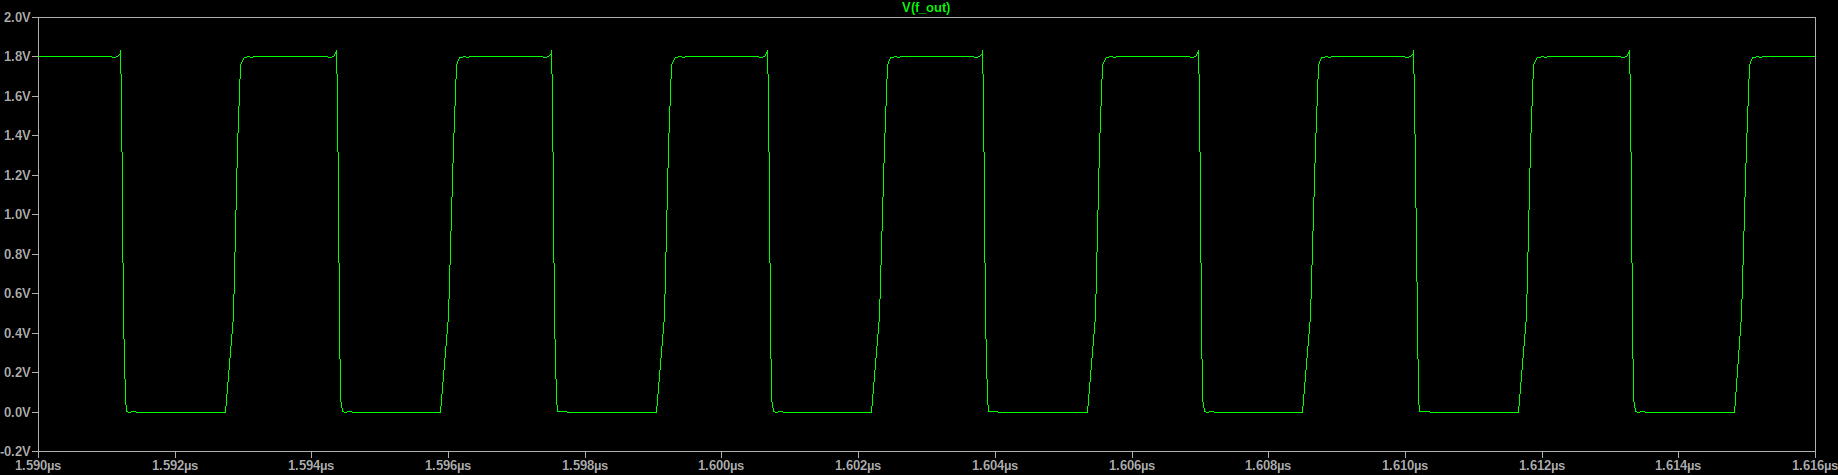
\includegraphics[width=0.9\textwidth]{figs/vco_op1.png}
	% \vspace{-0.3cm}
	\caption{output waveform of VCO}
	\label{fig:vco_sim}
\end{figure}


% \begin

% \subsection{LSTM network}

% \begin{figure*}[t]
% 	\centering
% 	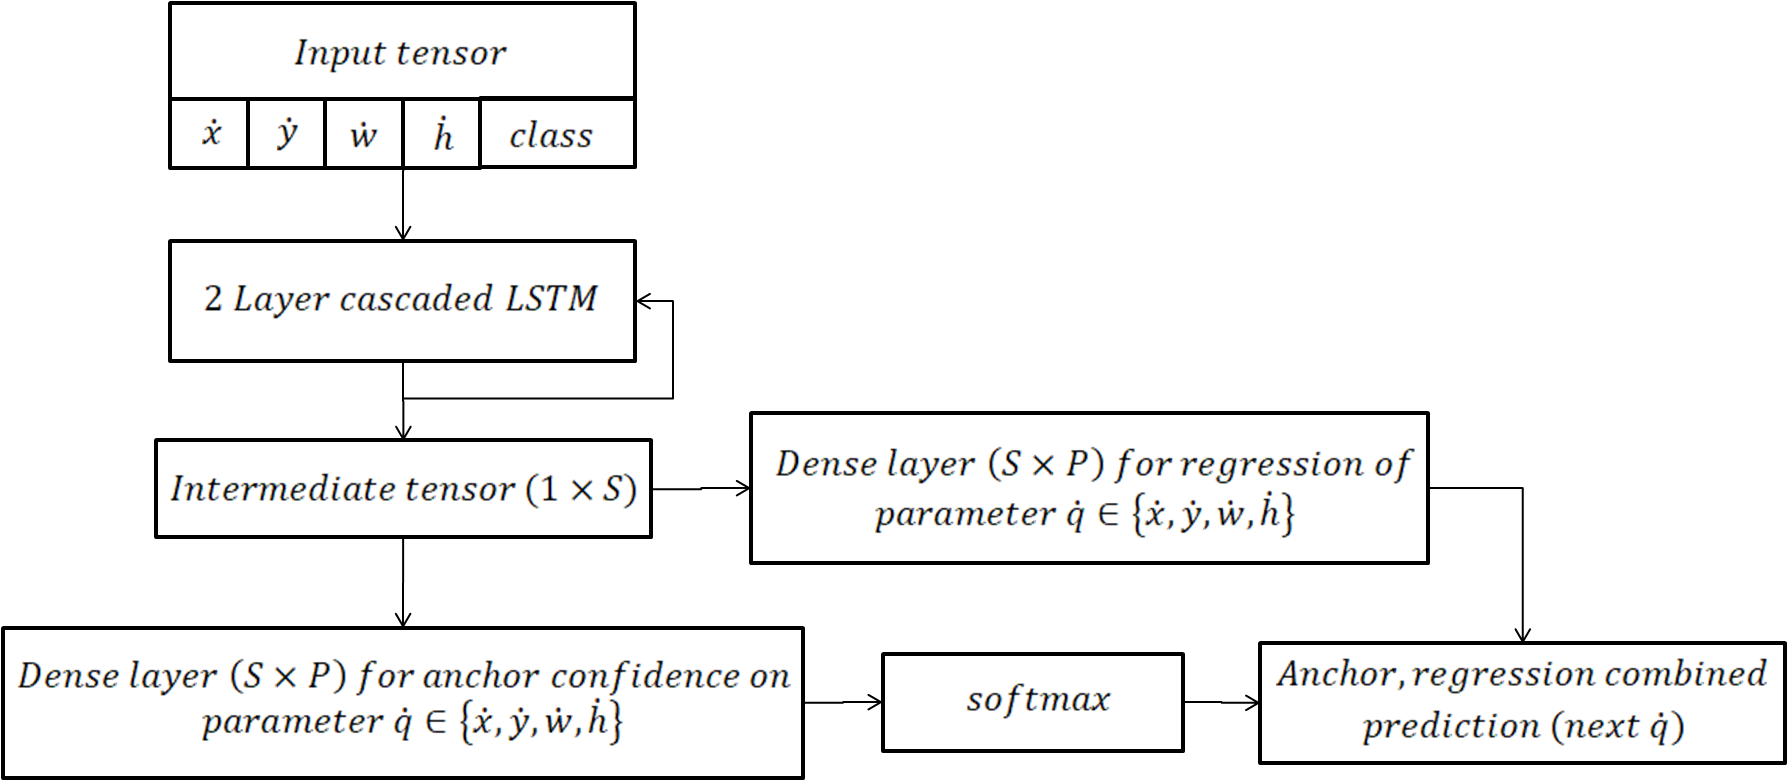
\includegraphics[ width=\textwidth]{figs/LSTM_network.png}
% 	\vspace{-0.5cm}
% 	\caption{Structure of the proposed LSTM network}
% 	\label{fig:LSTM_network}
% 	\vspace{0.5cm}
% \end{figure*}

% Consider a video as a sequence of image frames i.e. $V = I_{0},I_{1},...,I_{n}$ where $I_{k}$ s a matrix of fixed dimensions. Given detections $D = D_{0},D_{1},...,D_{n}$, for the objects present in each frame , where each  is a list of bounding box locations, class predictions, and other information corresponding to objects contained in the image , our goal here is to estimate the bounding box coordinates $B_{k+1,i}$ for each object in the following frame; $I_{k+1}$. Note that  $B_{k,i} = (x_{k,i},y_{k,i},h_{k,i},w_{k,i})$ where $x,y,h,w$ correspond to $x,y$ co-ordinates of centre, height and width of the bounding box for the $i^{th}$ object in the $k^{th}$ frame. Further, this system would operate in an online setting where at any given instance when time $t = k$, the frames, hence detections too are present only up to $I_{k}$ and $D_{k}$ respectively. Further the $i^{th}$ object will be consistent across consecutive frames (obtained using the output of the system) until the object disappears. The LSTM component can be viewed as a function $L$ with $L(D_{0},D_{1},...,D_{k}) = F_{k}$ where $F_{k}$ is a list of temporally aware feature maps $F_{k,i}$ corresponding to each object $i$ present within $D_{k}$. The remaining two functions; $C$ and $R$ correspond to classification (selecting anchor) and regression (estimating deviation from anchor) of the exact bounding box targets. Each bounding box datum $(x,y,h,w)$ is interpreted as a deviation from the previous time step $(\dot{x},\dot{y},\dot{h},\dot{w})$ which reduces the mean of those variables. Note that due to the discrete nature of data, $\dot{x} = x - x_{i-1}$ Using normalized co-ordinates ($x,y,h,w$ values divided by relevant image dimensions); this range will be within $(-1, 1)$ and an optimum number of anchors can be used to estimate this value as a classification problem. 
% \par Having laid down the classifications on to the targets, the required estimates from the classification function would be a one hot encoded tensor; $C_{out}$ of shape $(P, 4)$ for $P$ bins of anchors and 4 bounding box parameters. In our work, we use four bins; 0, 0.1, 0.5, 0.8 leading to a $(4, 4)$ tensor where the bin closest to the target value (ex: $\dot{x}$)  on each row would contain one and the rest zero. Each selected bin is an anchor located at a specific distance away from the next expected value for the parameter considered. The classification function can be presented as $C(F_{k,i}) = C_{out}$ The regression function output would be a similarly shaped tensor $R_{out}$. It is essential for the loss function to consider the nature of both the classification as well as regression outputs of the network. The overall model of estimator is illustrated in Figure \ref{fig:LSTM_network}. Here intermediate tensor corresponds to the temporally aware feature maps $F_{k,i}$ of the $i^{th}$ object and the system has four similar but separate instances of the dense layers to handle each parameter and that finally results in outputs $C_{out}$ and $R_{out}$. In essence the network estimates how far an object would move from its current position over the next time step. The $x,y$ components capture motion along the image axes while the $h,w$ components correspond to the motion along the depth axis as well as morphological change of the object to some extent. 
% \par When training; the loss function is obtained as a weighted sum of the classification and regression losses. The classification loss $LOSS_{C}$ is a simple cross-entropy loss function. The regression loss takes into account the sparse nature of the ground truth regression tensor. Here $\odot$ denotes the Hadamard product of two tensors or matrices.
% $$
% LOSS_{C} = -\sum(C_{out_{true}} \odot log(C_{out_{pred}})) \eqno{(1)}
% $$
% $$
% LOSS_{R} = argmax(C_{out_{pred}}) \odot L_{Huber}(R_{out_{pred}},R_{out_{true}}) \eqno{(2)}
% $$
% $$
% LOSS_{Total} = \lambda_{C}*LOSS_{C} + \lambda_{R}*LOSS_{R} \eqno{(3)}
% $$

% \begin{figure*}[t]
% 	\vspace{-0.7cm}
% 	\centering
% 	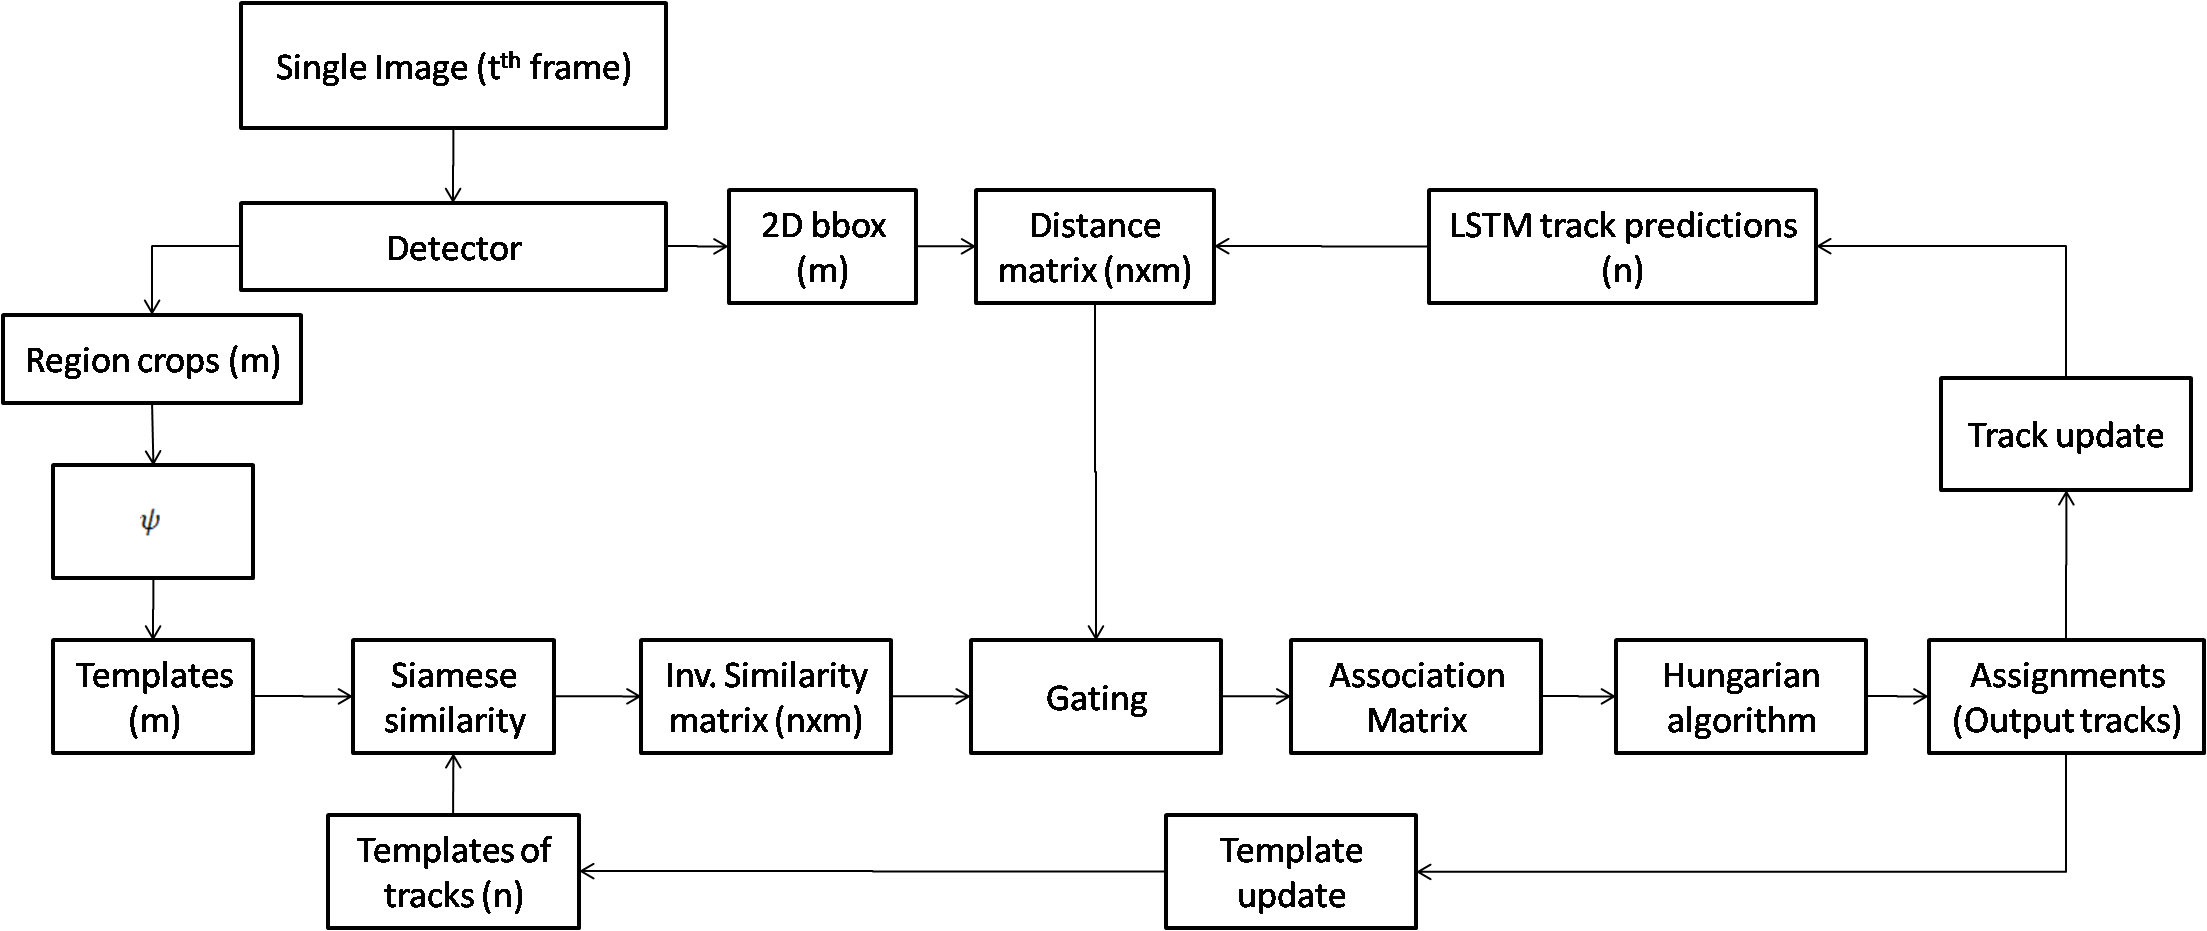
\includegraphics[ width=\textwidth]{figs/tracker.png}
% 	\vspace{-0.5cm}
% 	\caption{Overview of the overall 2D tracking system}
% 	\label{fig:tracker}
% 	\vspace{0.4cm}
% \end{figure*}

% \subsection{Appearance similarity}

% One of the most challenging problems in this context is handling occlusions. Object tracking with the use of a Kalman filter or an LSTM network to handle spatial coherence among tracks has been a common approach. However, the uncertainty involved in the track prediction increases when tracks are exposed to prolonged occlusions. Hence it is required to re-identify occluded tracks. Deep SORT \cite{DeepSiam:deepSort} introduces the use of feature vectors to define an appearance descriptor for the purpose of track re-identification. Results presented in this work have proven this to be a successful approach. However, this comes with the additional burden of training a large network for the sole purpose of re-identification of a particular class of objects. Hence this approach is not versatile for multi-class object tracking or for online implementation. Our approach has the ability to handle multiple classes of objects and can be implemented online with ease.
% \par The approach implemented in this paper involves the use of a Siamese network to determine the appearance consistency of tracks. The Siamese networks described in the SiamFC \cite{DeepSiam:SiamFC, DeepSiam:endrep} and SiamMask \cite{DeepSiam:siammask} works have proven to be highly successful in single object tracking but have not been incorporated into multi-object tracking yet. It has been trained on ImageNet datasets for similarity learning and can operate online. Thus, it can give a class independent measure for appearance consistency of tracks and therefore would be ideal for track re-identification. The network discussed in SiamFC \cite{ DeepSiam:endrep} extracts the features of the exemplar image and search image to produce a cross correlation map whose peak position corresponds to the position of the object in the exemplar image within the search image. Similarly, we use a Siamese network to produce a similarity measure between two images of the same size by building up templates through a convolution neural network (a convolution function as in \cite{ DeepSiam:endrep} shown in template generation step through Figure \ref{fig:LSTM_association})
% \par The cross-correlation map produced by the Siamese network is passed through a similarity function to produce the similarity score, or more accurately an appearance cost. The similarity function in this context is defined as follows,
% $$
% Appearance \; Cost = A \exp(-k\ \sum f(x,y)) \eqno{(4)}
% $$
% where $f(x,y)$ is the cross correlation value at $x,y$ position in the cross correlation map and $A,k$ are tunable parameters.


% \subsection{Track Association}

% The track association is based on the association cost which depends on the appearance cost (from the Siamese network) as well as a distance metric. The distance metric is the measurement of how far the detection bounding box is from the bounding box of a track predicted by the LSTM. The distance metric between two bounding boxes is defined based on the IOU distance (intersection over union) between the bounding boxes. Let $ a_{i,j},c_{i,j},d_{i,j}$ represent the association cost, appearance cost and the distance metric between the $i^{th}$ detection and the $j^{th}$ track.
% $$ 
% a_{i,j} = 
% \begin{cases} 
% c_{i,j} \; if \; d_{i,j} < T \\
% K \; if \; d_{i,j} \geq T \\ 
% \end{cases}
% \eqno{(5)}
% $$
% where $K$ is the gating constant and $T$ is the gating threshold. Track association is treated as an assignment problem and is carried out using the Hungarian algorithm \cite{DeepSiam:hungarian} following very closely the approach discussed in Deep SORT \cite{DeepSiam:deepSort}.

% \subsection{Overall online tracking system}

% The Siamese network for similarity measurement is implemented in two stages. The first stage involves producing feature maps (templates) for detections in the current frame and the next stage involves producing cross correlation maps by convolving the detection templates with track templates and generating an appearance cost matrix between track, detection pairs in that frame. These two stages have been isolated to improve the efficiency of the approach.
% \par In a given frame, a crop of the bounding box corresponding to each detection is extracted. These crops are resized to 127x127 and passed through the first stage of the Siamese network to generate templates for each detection in that particular frame. These templates are passed through the second stage of the Siamese network along with the templates of tracks in order to generate a matrix of appearance costs. This cost matrix is gated according to the distance metric and subjected to the Hungarian algorithm to obtain track assignments for the detections.
% \par For matched track, detection pairs; the template of the track is updated using a rolling average between the track’s current template and the template of the detection which was matched to it,
% $$
% temp_{track} = \gamma * temp_{track} + (1 - \gamma) * temp_{det} \eqno{(6)}
% $$
% where $\gamma$ is the occluded percentage of the matched detection and defined as the maximum of the Intersection over Union values (IoU) between the detection bounding boxes and the bounding box of the matched detection which is one when fully occluded and zero when the object is fully visible. Therefore, when the matched detection is fully visible, it replaces the template of the track with the template of the matched detection and when the matched detection is fully occluded, it does not update the template of the track so as not to contaminate the template with the features from occlusions.
% \par Deletion of tracks and addition of new tracks is carried very similar to the approach carried out in the Deep SORT \cite{DeepSiam:deepSort} work.

% \subsection{Extensibility to BEV space}
% The seemingly simple but effective fact that ‘overlapping in BEV space projections cannot happen for the objects detected and predicted in 3D is exploited here through a constrained optimization problem. This work relates to the possible improvements that could be done on the system and detailed in \ref{chapter:appendix1}.

% \subsection{LSTM based data association for end to end trainability}

% \begin{figure*}[t]
% 	\centering
% 	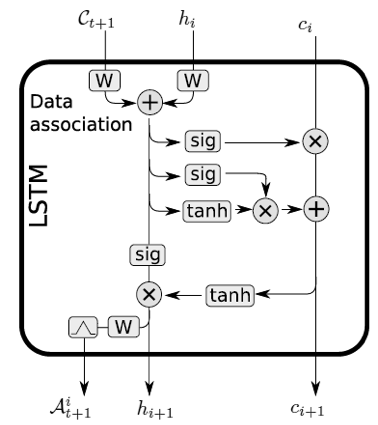
\includegraphics[width=0.5\textwidth]{figs/lstm_associate.png}
% 	\vspace{-0.3cm}
% 	\caption{Association LSTM}
% 	\label{fig:LSTM_association}
% 	\vspace{0.5cm}
% \end{figure*}

% The multi object tracker network uses the Hungarian algorithm for data association where this algorithm is a definite setup having an algorithmic complexity of $O(n^3)$. However the system cannot be back propagated through this implementation due to the fact that Hungarian algorithm is not differentiable. There are approaches from probabilistic view points as in \cite{russel}  and with learning perspective as presented in \cite{DeepSiam:multitarget} for obtaining a data driven system. Several experiments were conducted with data association on MOT tracking dataset based on the methodology presented in [19]. The system developed is shown in Figure \ref{fig:LSTM_association} and was designed from scratch using tensorflow API. The system was designed initially to handle and check the repeated lengthy tracks in the dataset without the intervention of birth and death processes. Here the system is getting trained to build up a probability matrix $A_t$ which presents associations at time t. Thus $A_t^i=[p_{i,1},p_{i,2},p_{i,3},\ldots,p_{i,m},p_{i,m+1}]$ where  $p_{i,j}$ represents the probability of $i^{th}$  target being denoted by $j^{th}$ measurement out of m measurements for the frame (i.e. m detections).
% Here 
% $\sum_{j=1}^{m+1}p_{i,j}=1$ which is achieved by using softmax on the row.

% The excess column presented by the last probability shows the probability that none of measurements being matched for the respective track and this track will potentially be terminated in next stages of the process.
% The input $C_t\in R^{N\times M}$ is the matrix created through the second norm between the state vector $x_i$ of the target and the measurement having feature vector $z_j$.
% Therefore, $C_t^{i,j}=\ x_i-z_j^2$

% Negative log likelihood loss was used as the loss function for training. 


% \section{Panoptic Segmentation}
% Our work is concentrated to the assignment of a semantic label and an instance label for each pixel in an image using a novel approach of incorporating bipartite potentials to improve the segmentation accuracy.

% \subsection{Background: Conditional Random Fields}

% Conditional Random Fields (CRFs) are a class of statistical modeling method used for structured prediction. A CRF, used in the context of pixel-wise label prediction, models pixel labels as random variables that form a Markov Random Field (MRF) when conditioned upon the image. CRFs have primarily been used in computer vision for semantic image segmentation. In this setting, CRFs encourage the desirable properties of a good segmentation, such as the spatial consistency (e.g. spatially neighboring pixels should have the same label) and color consistency (e.g. a semantic segmentation boundary should correspond to a edge in the image) through various energy functions used in the formulation. A CRF formulation usually has energy terms arising from an imperfect classifier (sometimes known as the unary energy) and energy terms encouraging the consistency properties of the segmentation (sometimes known as the pairwise energy). Some semantic CRF models also include higher order energy terms to encourage higher order consistency properties such as consistency of the labeling within super-pixels~\cite{arnab_eccv_2016}.

% Once an appropriate energy function is formed, the optimal labeling is found as the labeling that minimizes the CRF energy (or equivalently, maximizes the probability). This is known as the inference of the CRF. The exact inference of a CRF with dense pairwise connections is intractable and hence approximate inference methods such as mean field variational inference has to be utilized to solve the CRF in reasonable time~\cite{densecrf}. For a detailed treatment of CRFs, the reader is referred to~\cite{Koller_book}. 

% \subsection{Bipartite CRFs}
% \label{sec:body}
% We propose a CRF formulation with bipartite random variables to capture interactions between semantic labels and instance labels. Inference of this CRF gives the jointly most probable semantic and instance segmentation (and therefore, the panoptic segmentation) for a given image. 

% For each pixel $i$, define a pair of discrete random variables $(X_i, Z_i)$ to denote its semantic label and the instance label, respectively. For each $i$, $X_i$ can take values in $\mathcal{L} = \{l_1, l_2, \dots, l_L\}$, where each $l_j$ is a semantic label and $L$ is the number of semantic labels (includes both stuff and thing classes). Therefore, $\mathcal{L} = \Lstuff \cup \Lthings$, where $\Lstuff$ is the set of stuff class labels and $\Lthings$ the set of thing class labels. Similarly, for each $i$, $Z_i$ can take values in $\mathcal{T} = \{\inst_0, \inst_1, \dots, \inst_{\Ninst} \}$, where $\Ninst$ is the number of instances detected in the image, and the label $\inst_0$ is reserved to represent the ``no instance'' case (the pixel belongs to a stuff class).  


% Let $\X = [X_1, X_2, \dots, X_N ]$ and $\Z = [Z_1, Z_2, \dots, Z_N
% ]$, where $N$ is the number of the pixels in the image. A joint assignment $(\x, \z)$ to these two random vectors $(\X, \Z)$ gives a unique semantic label and an instance label to each pixel $i$, and therefore represents a panoptic segmentation of the image. Note that, $\x \in \mathcal{L}^N$ and $\z \in \mathcal{T}^N$. In this work, we discuss the probability of such assignments and formulate the probability distribution function so that the ``good'' panoptic segmentation will have a high probability. We then perform inference on this formulation to find the assignment that maximizes the probability to obtain the best panoptic segmentation.

% The probability of a panoptic segmentation $(\x, \z)$, given the image $I$, can be modeled as a Gibbs distribution of the following form:
% \begin{equation}
% \label{eqn:prob}
% \Pr(\X = \x, \Z = \z|I) = \frac{1}{\mathcal{Z}(I)}\exp(-E(\x, \z|I)),
% \end{equation}
% where $\mathcal{Z}(I) = \sum_{(\x,\z)} \exp(-E(\x, \z|I))$, is a normalization constant, sometimes known as the partition function. The term $E(\x, \z|I)$ is known as the energy of the configuration $(\x, \z)$. Hereafter, we drop the conditioning on $I$ in the notation for brevity. The energy of our bipartite CRF is defined as follows:

% \begin{equation}
% \label{eqn:energy}
% \begin{split}
% E(\x, \z) =& \sum_i\phi(x_i) + \sum_{i < j}\Phi(x_i, x_j) \;+ \\
% & \sum_i\psi(z_i) + \sum_{i < j}\Psi(z_i, z_j) \; + \\
% & \sum_i\omega(x_i, z_i) + \sum_{i < j}\Omega(x_i, z_j),
% \end{split}
% \end{equation}
% where $x_i$ and $z_i$ are the elements of the vectors $\x$ and $\z$, respectively. The meaning of each term will be described in detail below. Note that, since a ``good'' panoptic segmentation should have a high probability, it should have a low energy. Various terms in Eq.~\eqref{eqn:energy} should therefore encourage a good panoptic segmentation by penalizing disagreements with our prior knowledge about a consistent panoptic segmentation. % Roughly speaking, the energy terms represent negative log probabilities. 

% \subsection{Semantic Component of the CRF}
% In the following, we discuss the first two term of the energy function in Eq.~\eqref{eqn:energy}. The first term encourages the semantic segmentation result to be consistent with the initial classifier.
% \begin{equation}
% \phi(X_i = x_i) = - \log(\Pro(X_i = x_i)),
% \end{equation}
% where $\Pro(.)$ is the classifier probability score for the semantic segmentation. 

% The second term in Eq.~\eqref{eqn:energy} encourages the smoothness of the semantic labeling:
% \begin{equation}
% \label{eq:similarity}
% \Phi(X_i = x_i, X_j = x_j) = \mu(x_i, x_j) \operatorname{Sim_\Phi}(i, j),
% \end{equation}
% where $\mu: \mathcal{L} \times \mathcal{L} \to \mathbb{R}$ is the label compatibility function, and $\operatorname{Sim_\Phi}(i, j)$ is a similarity measure between the pixels $i$ and $j$. This term penalizes assigning different labels to a pair of pixels that are ``similar". Following \cite{densecrf}, we use a mixture of Gaussians as the similarity measure. Therefore,
% \begin{equation}
% \label{eqn:kernels}
% \operatorname{Sim_\Phi}(i, j) = \sum_m w_{\Phi, m} \exp\left(-\frac{\|\vec{f}_i^{(m)} - \vec{f}_j^{(m)}\|^2}{2\sigma_{\Phi,m}^2}\right)
% \end{equation}
% where $\mathbf{f}_i$ is a feature vector for pixel $i$ containing information such as its spatial location and bilateral features (RGB + spatial coordinates). We use the same spatial and bilateral features used in~\cite{densecrf}.
% \subsection{Instance Component of the CRF}

% For the instance classification, we also assume the existence of an initial classifier, such as Mask R-CNN, that provides a confidence score for each instance at each pixel. Note that Mask R-CNN provides fixed-size instance segmentation predictions with respect to the bounding boxes of the detections. However, these predictions can be easily mapped to the full image by using bilinear interpolation and trivial coordinate transforms.

% In the following, we use $z_i \in \{\inst_0, \inst_1, \dots, \inst_\Ninst \}$, where $\Ninst$ is the number of instances detected in the image. The label $\inst_0$ is reserved for the special case where the pixel does not belong to an instance, i.e., it belongs to a stuff class.

% Similar to the semantic segmentation case, the third term in Eq.~\eqref{eqn:energy} encourages the panoptic segmentation to be consistent with the instance classifier probabilities $\Pro$:
% \begin{equation}
% \psi(Z_i = z_i) = - \log(\Pro(Z_i = z_i)).
% \end{equation}

% The fourth term in Eq.~\eqref{eqn:energy} encourages instance label consistency across the whole image by penalizing assigning different instance labels to similar pixels:
% \begin{equation}
% \Psi(Z_i = z_i, Z_j = z_j) = [z_i \neq z_j] \operatorname{Sim_\Psi}(i, j).
% \end{equation}
% The compatibility transform in this case is fixed to be $[z_i \neq z_j]$, where $[.]$ is the Iverson bracket. The similarity measure $\Sim_\Psi$ has a similar form to Eq.~\eqref{eqn:kernels}. %Intuitively, this term encourages \emph{similar} pixels to have the same instance label.

% \subsection{Cross Potentials in the CRF}
% An important contribution of this paper is the introduction of cross potentials between the semantic segmentation and instance segmentation. The semantic segmentation and the instance segmentation are highly related problems and therefore the solutions should agree: the semantic label at any pixel has to be compatible with the instance label at that pixel. For example, if the instance labeling says that the pixel $i$ belongs to an instance of a person class, the semantic label at pixel $i$ should also have the person label. If the initial classifier results for the instance segmentation and the semantic segmentation do not agree, one of them should correct itself depending on the interactions of other terms in the CRF.

% The first cross potential term (the fifth term in Eq.~\eqref{eqn:energy}), encourages instance label and the semantic label at a given pixel to agree:
% \begin{equation}
% \omega(X_i = x_i, Z_i = z_i) = f(x_i, \cl(z_i)).
% \end{equation}
% Here, $\cl(z_i)$ is the class label of the instance $z_i$ with $\inst_0$ mapped to a special class $\operatorname{null}$. Note that, for all valid instances, the class label can be obtained from the instance classifier (e.g. Mask R-CNN). The function $f(., .): (\mathcal{L}, \Lthings \cup \{\operatorname{{null}}\}) \to \mathbb{R}^+_0$, captures the cost of incompatibility and is defined as follows: 
% \begin{equation}
% \label{eqn:cross_compat}
% f(x_i, \cl(z_i)) = \begin{cases}
% 0,\;\;\text{if}\;x_i = \cl(z_i)\\
% 0,\;\;\text{if}\;x_i \in \mathcal{L}_{\text{stuff}}\;\text{and}\;\cl(z_i) = \operatorname{null}\\
% \eta(x_i, \cl(z_i)),\;\; \text{otherwise}.
% \end{cases}
% \end{equation}
% The above function covers three cases: 1) If the semantic label and the class label of the instance label match, there will be no penalty for such assignment since there is no incompatibility in this case. 2) If the semantic segmentation assigns a stuff label and the instance segmentation assigns $\inst_0$ label, there will be no penalty in that case either. 3) If the semantic label and the instance label mismatch, there will be a penalty with the magnitude decided by the function $\eta(., .): \Lthings \cup \{\operatorname{null}\} \times \Lthings \cup \{\operatorname{null}\} \to \mathbb{R}^+$. This function is learned from data as described in Section~\ref{sec:infer}.

% The last term in Eq.~\eqref{eqn:energy}, encourages the consistency of semantic label and the instance label among similar looking pixels and has the form:
% \begin{equation}
% \Omega(X_i = x_i, Z_j = z_j) = f(x_i, \cl(z_j))\; \operatorname{Sim_\Omega}(i, j),
% \end{equation}
% where each symbol has the meaning described above.


% \subsection{Inference and Parameter Optimization}
% \label{sec:infer}
% The best panoptic segmentation given the model described in Section~\ref{sec:body} is the assignment $(\x, \z)$ that maximizes the probability in Eq.~\eqref{eqn:prob}. However, since the graphical model used in BCRF has dense connections between the pixels, the exact inference is infeasible. We therefore use an approximate parallel mean field inference algorithm following~\cite{densecrf}.

% In this setting, the joint probability distribution is approximated by the product of marginal distributions:
% \begin{equation}
% \label{eq:q_approx}
% \Pr(\X=\x, \Z=\z) \approx \prod_i Q_i(x_i)\,R_i(z_i),
% \end{equation}
% where $Q_i(x_i) = \Pr(X_i = x_i)$ and $R_i(z_i) = \Pr(Z_i = z_i)$ are the marginal distributions. Out of all the distributions that can be written down in this factorized form, the closest distribution to the original joint distribution is found by minimizing the KL divergence~\cite{Koller_book, densecrf}. For our BCRF formulation, this results in the iterative algorithm detailed in Algorithm~\ref{alg:infer}.

% To make our model flexible, we deliberately include a number of parameters in the BCRF model, which we automatically learn from the training data. More specifically, the BCRF model has the following parameters:
% \begin{enumerate}
% 	\item Weight multipliers for different energy terms: each term in Eq.~\eqref{eqn:energy} is multiplied with a weight parameter, which decides the relative strength of the term. This parameterization helps learn the optimal combination of different energies in the CRF. For example, if the initial semantic segmentation model has better accuracy than the instance segmentation model, the $\phi$ unary energy might be weighted more than the $\psi$ unary energy.
	
% 	\item Parameters for similarity functions: Each similarity function $\Sim_X(i, j)$ of the form shown in Eq.~\eqref{eq:similarity} has its own parameters. These learn the relative strength of spatial and appearance consistency of the panoptic segmentation.
	
% 	\item Label compatibility matrices: The two functions $\mu(., .)$ and $\eta(., .)$ are initialized to have a zero cost for a pair identical labels and a fixed cost for any combination of two different labels. They are then given the freedom to automatically learn the relative penalty strengths for different label combinations.
% \end{enumerate}


% \subsection{BCRF in a Deep Network}
% In this section, we discuss how BCRF can be used in a deep network. In~\cite{Zhen_ICCV15_CRFRNN}, authors showed that, in the semantic segmentation setting, mean field inference of a CRF with Gaussian pairwise potentials can be formulated as a Recurrent Neural Network (RNN). Since our BCRF also uses an iterative mean field algorithm of similar nature, it is readily adaptable into the RNN based inference described in~\cite{Zhen_ICCV15_CRFRNN}. Therefore, BCRF can be a first-class citizen of a deep network performing panoptic segmentation. Importantly, this formulation allows automatic optimization of the BCRF parameters described in Section~\ref{sec:infer}, using backpropagation and a gradient descent algorithm such as stochastic gradient descent (SGD). This is a major advantage since it allows us to increase the number of parameters used in BCRF, and hence increase its flexibility, without adding to the burden of manual parameter optimization.

% In the current state-of-the-art methods, semantic segmentation and instance segmentation are solved with different network architectures with complimentary strengths. The BCRF formulation given a systematic way of combining these strengths in a probabilistic framework. Such an example usage of BCRF is shown in Figure~\ref{fig:bcrf_net}. The CNN feature extractor here can be a common backbone network such as ResNet-101 or ResNeXt. The semantic segmentation branch is usually a fully convolutional network that is capable of seeing a wide field of view, where as the instance segmentation branch is a region-proposal based network such as Mask R-CNN. The semantic segmentation branch's output is taken as the $\phi$ unary potential input to the BCRF, and instance segmentation branch's output as the $\psi$ unary potentials. In addition, the raw image is also fed into the BCRF to derive the similarity functions $\Sim_X(., .)$ using the pixel locations and the RGB values. 

% During the training of the network, in the forward pass, BCRF inference is performed using Algorithm~\ref{alg:infer}. A suitable loss function for panoptic segmentation can then be used at the output of the network. In the backward pass, differentials with respect to the loss function will be passed into the BCRF inference to optimize various parameters used in the BCRF model. Importantly, during the backward pass, after BCRF inference, the error differentials can be passed on to the semantic branch and the instance branch both to optimize their parameters, and subsequently, the feature extractor CNN's parameters. Therefore, the whole network, including the BCRF component, can be jointly trained.




  % \chapter{Results \& Analysis}
\label{chapter:results}
\section{Results}
The circuit schematica was captured and simulated using the LTSpice software. The simulation was performed to analyze the performance of the circuit and to verify its functionality. The results of the simulation are presented in this section.
The simulation was performed using the following parameters:
\begin{itemize}
    \item Supply voltage: 1.8V
    \item Input frequency: 5MHz
    \item Input amplitude: 1.8V
    \item Frequency Multiplication Factor: 8
\end{itemize}
The simulation results are shown in the following figures. The first figure shows the 
output waveform of the circuit.output waveform of the circuit, which is a square wave. The output waveform is shown in Figure \ref{fig:output_waveform}.
\begin{figure}[H]
    \centering
    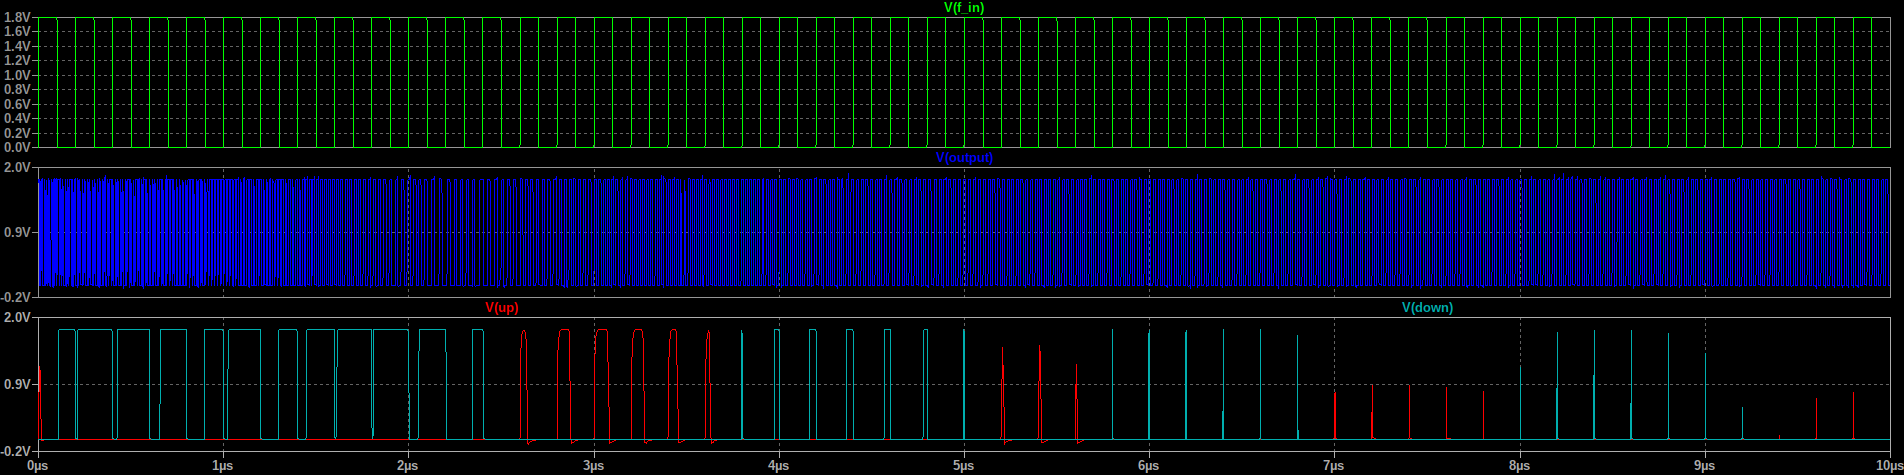
\includegraphics[width=1\textwidth]{figs/finalop5MHz.png}
    \caption{Output Waveform of PLL}
    \label{fig:output_waveform}
    \vspace{0.5cm}
\end{figure}
We can observe the phase locking of the output waveform with the input waveform in the Figure \ref{fig:output_waveform_phaselocking}.
\begin{figure}[H]
    \centering
    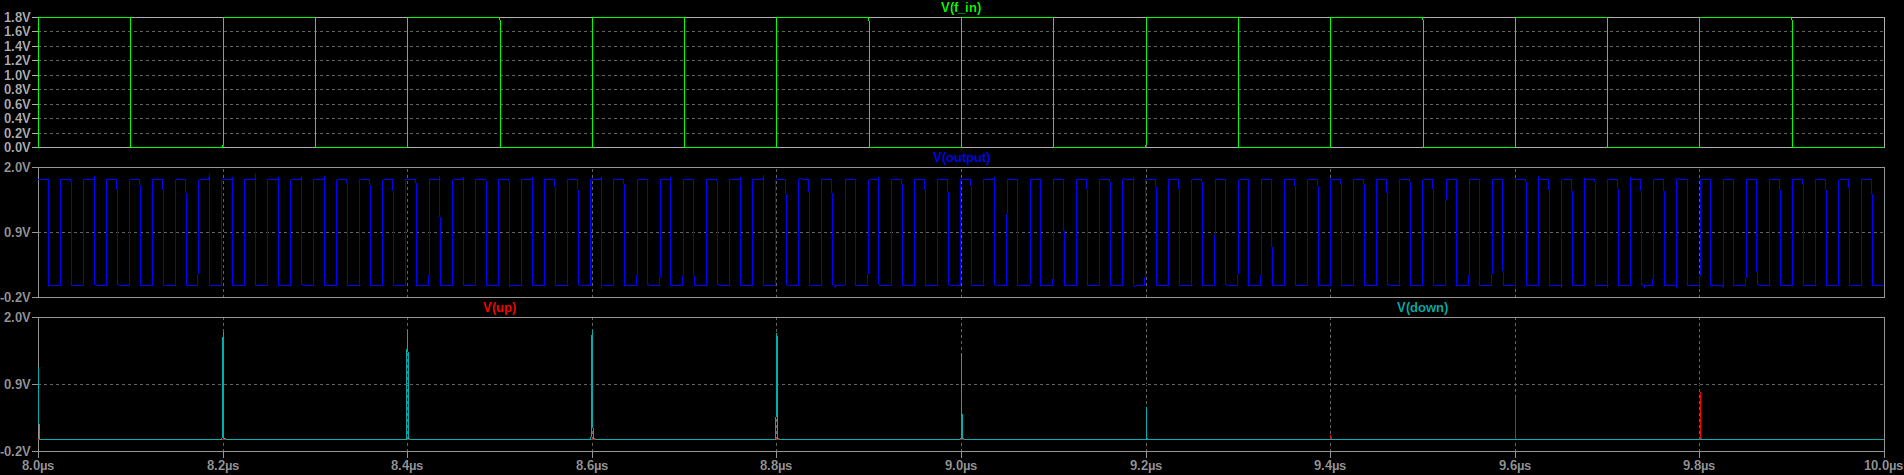
\includegraphics[width=1\textwidth]{figs/finalopphaselock.png}
    \caption{Magnified Output Waveform of PLL}
    \label{fig:output_waveform_phaselocking}
    \vspace{0.5cm}
\end{figure}
The second figure shows the output frequency spectrum of the circuit. The output frequency spectrum is shown in Figure \ref{fig:output_frequency_spectrum}. The output frequency spectrum shows the frequency components of the output waveform.

\begin{figure}[H]
    \centering
    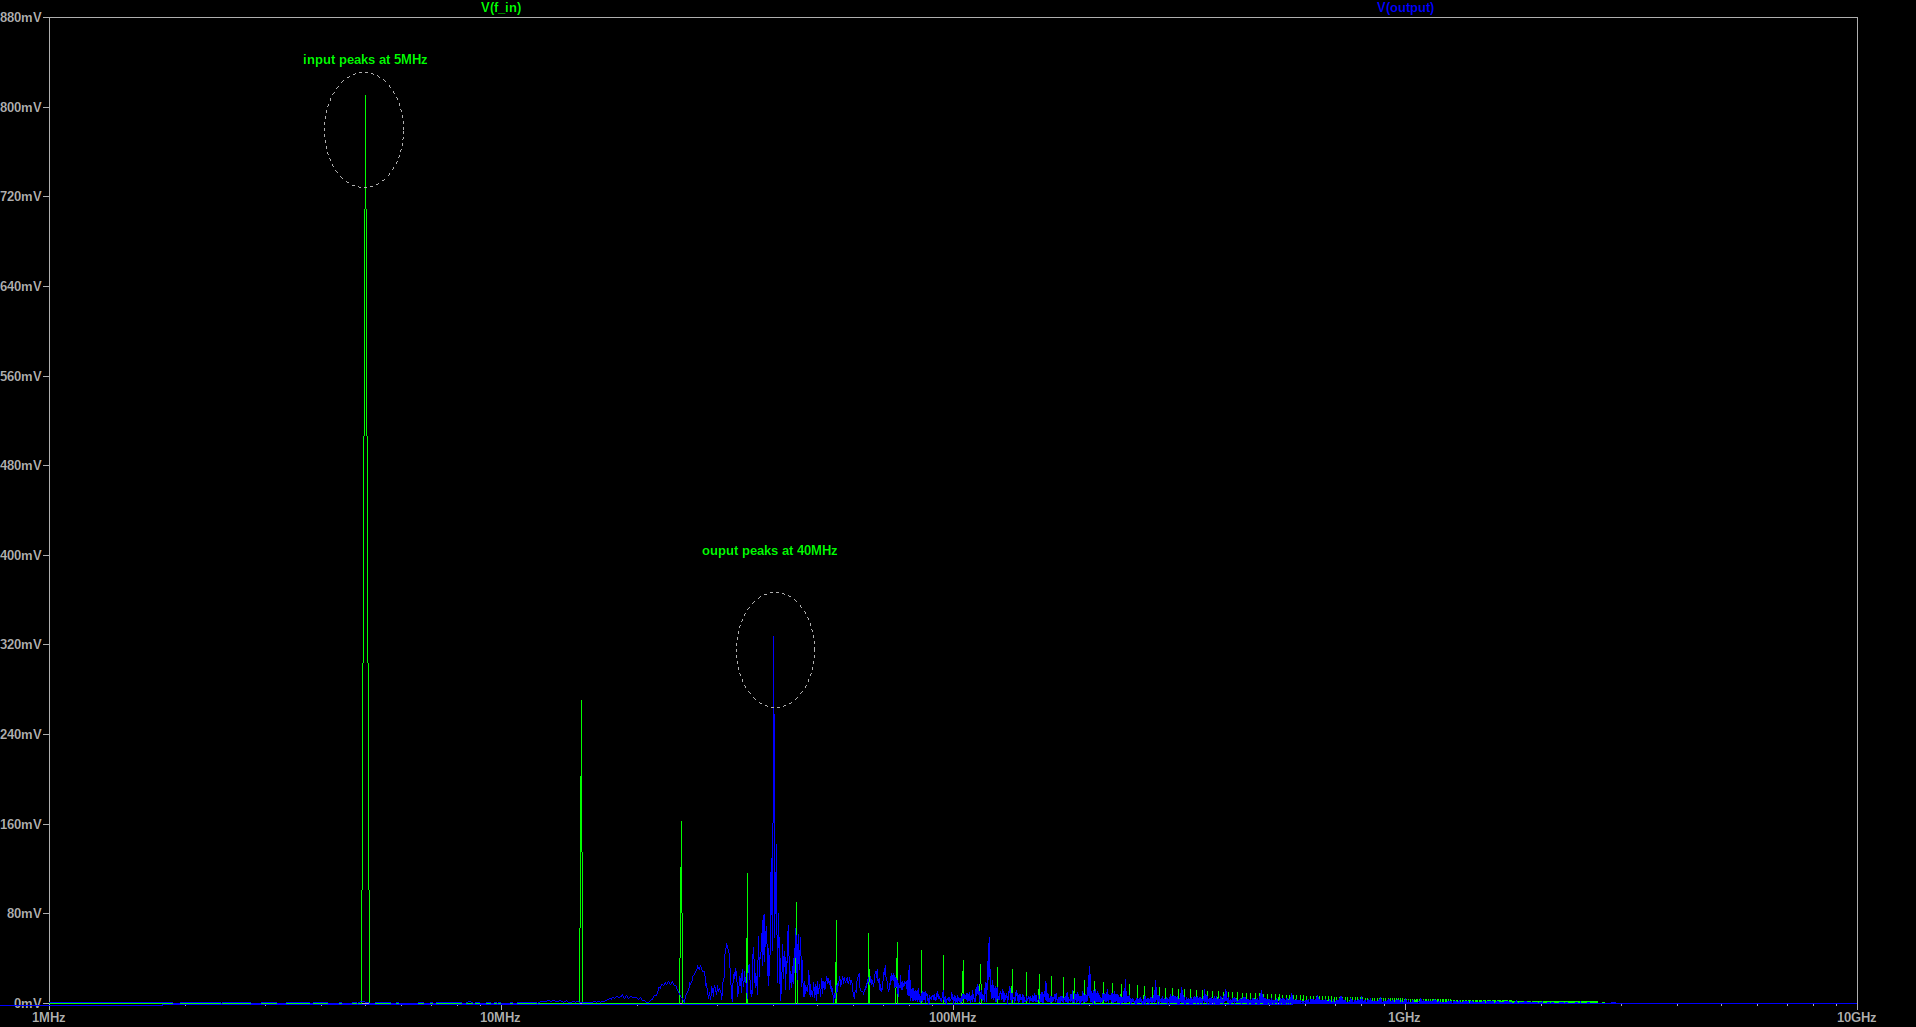
\includegraphics[width=1\linewidth]{figs/pllfftop2.png}
    \caption{Output Frequency Spectrum of PLL}
    \label{fig:output_frequency_spectrum}
    \vspace{0.5cm}
\end{figure}

Hence The following results were obtained from the simulation:
\begin{itemize}
    \item The output frequency is 40MHz, which is 8 times the input frequency of 5MHz.
    \item The output waveform is a square wave with a duty cycle of 50\%.
    \item The output amplitude is 1.8V, which is for whicht the VCO is designed for.
    \item The output frequency spectrum shows the frequency components of the output waveform, which are at 40MHz and its harmonics.
    \item Phase locking of the output waveform with the input waveform is observed.
\end{itemize}  

\section{Analysis}
Batch simulation was performed to analyze the performance of the circuit. The simulation was performed for different input frequencies. 
The input frequencies were varied from 1GHz to 500KHz. The output frequency was measured for each input frequency. The results of the simulation are shown in the following table \ref{tab:simulation_results}.

\begin{table}[H]
    \centering
    \begin{tabular}{|c|c|c|}
        \hline 
        \textbf{Simulation No.} & \textbf{Input Frequency} & \textbf{Output Frequency} \\
        \hline
        1 & 1GHz & --\\
        2 & 900MHz & --\\
        3 & 800MHz & --\\
        4 & 700MHz & --\\
        5 & 600MHz & --\\
        6 & 500MHz & --\\
        7 & 400MHz & --\\
        8 & 300MHz & --\\
        9 & 200MHz & --\\
        10 & 100MHz & --\\
        11 & 90MHz & --\\
        12 & 80MHz & --\\
        13 & 70MHz & --\\
        14 & 60MHz & --\\
        15 & 50MHz & --\\
        \hline
    \end{tabular}
    \caption{Simulation Results}
    \label{tab:simulation_results}
\end{table}
The output frequency was measured for each input frequency and observed through the ouput frequency Spectrum With respect to its input frequency spectrum achived through FFT view tool on LTSpice as shown in Figure \ref{fig:batch_input_frequency_spectrum} \& \ref{fig:batch_output_frequency_spectrum}.

Hence we can arrive to the conclusion the PLL able retain its functionality for the input frequency ranging from 22.5MHz to 3.75MHz.
\begin{figure}
    \centering
    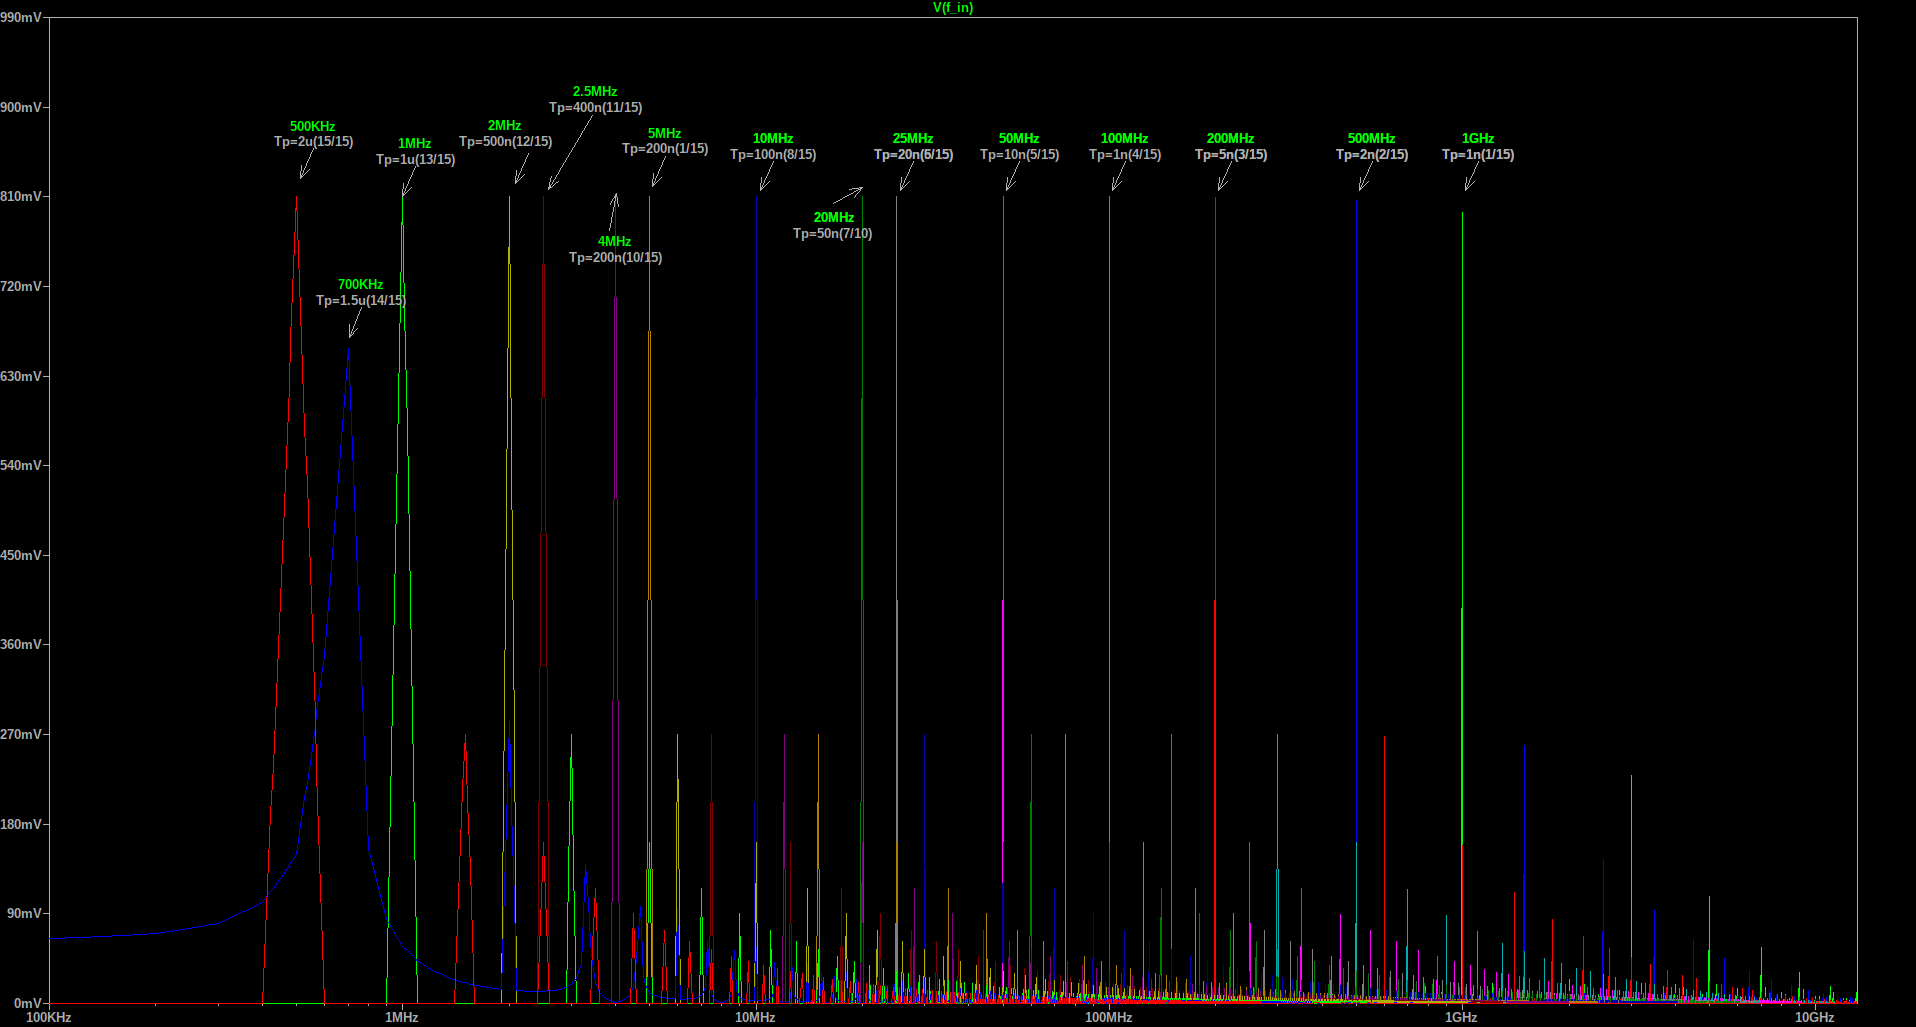
\includegraphics[width=1\linewidth]{figs/finfft.png}
    \caption{Output Frequency Spectrum of PLL}
    \label{fig:batch_input_frequency_spectrum}
    \vspace{0.5cm}

\end{figure}
\begin{figure}
    \centering
    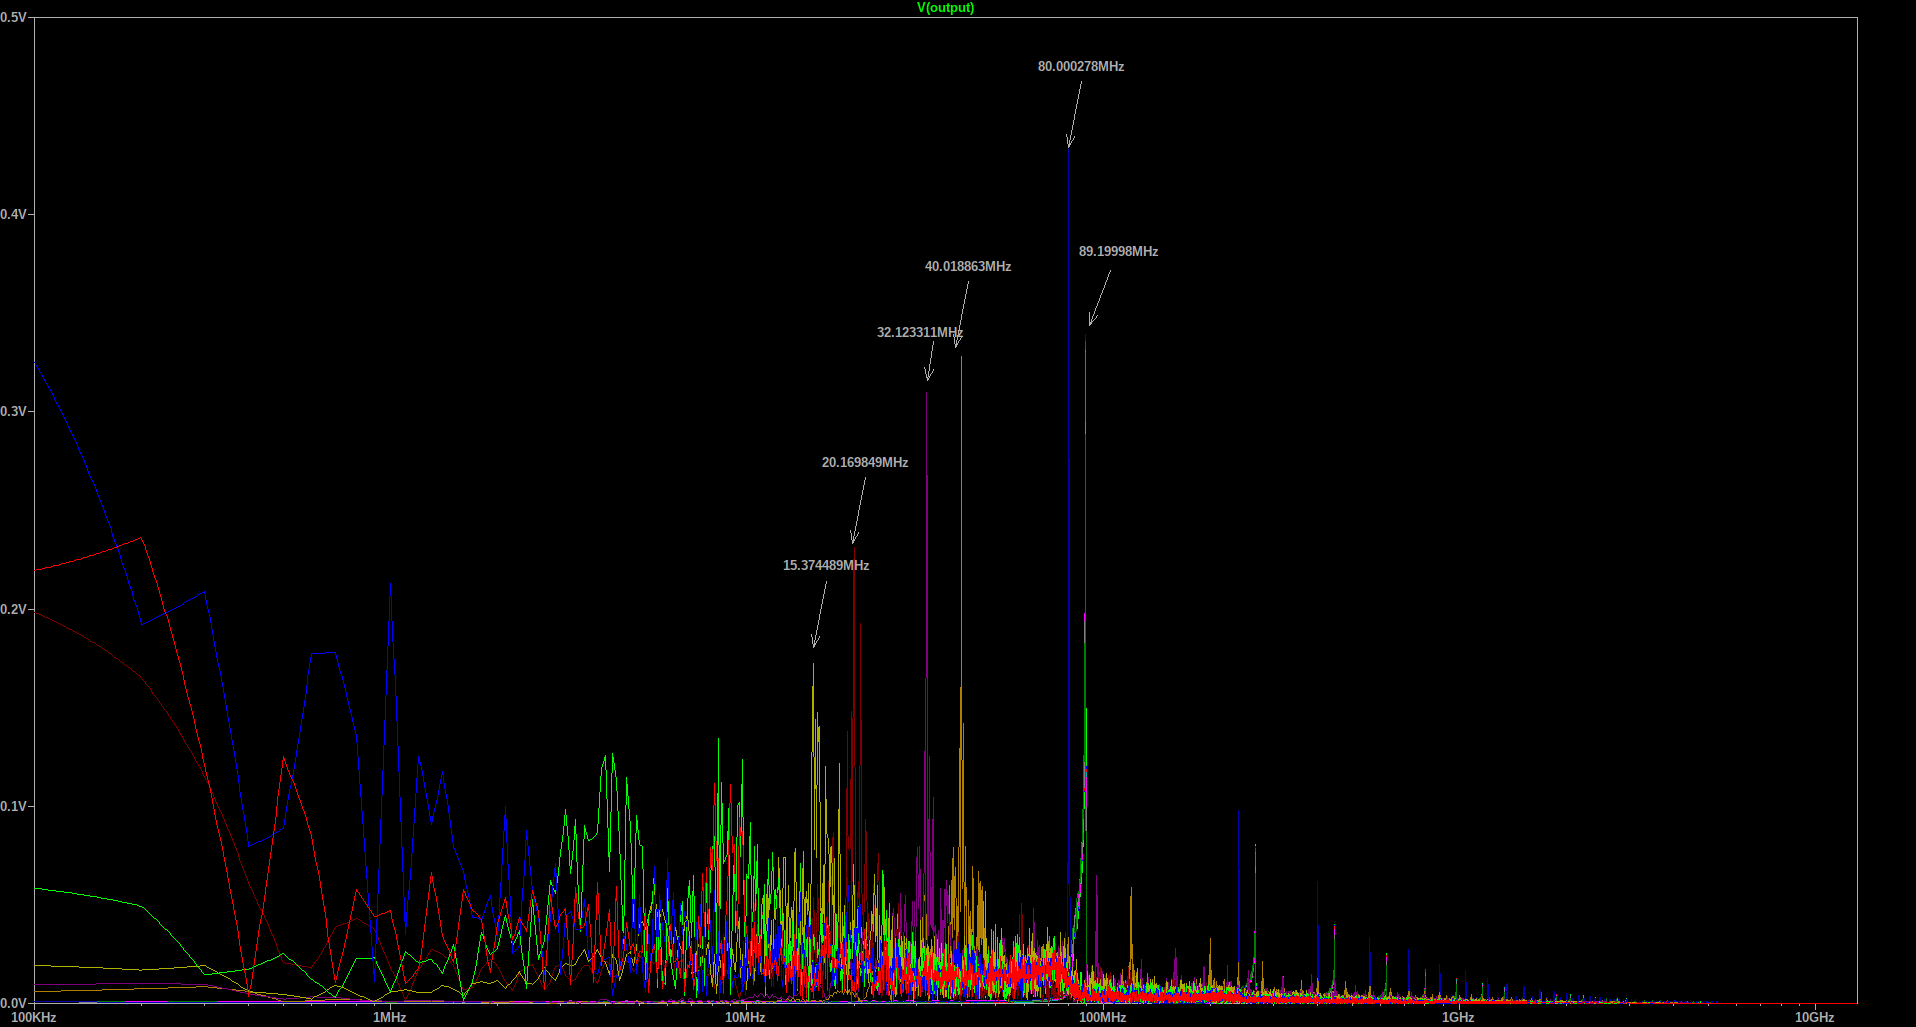
\includegraphics[width=1\linewidth]{figs/foutfft.png}
    \caption{Output Frequency Spectrum of PLL}
    \label{fig:batch_output_frequency_spectrum}
    \vspace{0.5cm}
\end{figure}
  % \chapter{Discussion and Conclusion}

We propose two components essential for autonomous systems that interact with their surrounding environments. These are in fact two of the key computer vision problems that have been attempted for a long time. 

Firstly, we present an end-to-end system capable of performing multi-object tracking by combining a range of advances in object detection and reidentification along with our novel architectures and loss functions. Further, we work on a novel step by building a separate LSTM branch to estimate the similarity feature map for the next time step of a given track. The Siamese Networks may be viewed as a two-step version of our extension, whereas this replacement with an LSTM is more of a generalized version capable of generating a better feature set. The key expectation with this addition is the overcoming of identity switches and lost tracks in the case of occlusions. Appearance features tend to change significantly during an occlusion, especially when an object undergoes rotations, and our extension overcomes this by modeling the appearance changing pattern over time. 

Thereafter, we proposed a probabilistic graphical model based framework for panoptic segmentation. Our CRF model with two different kinds of random variable, named Bipartite CRF or BCRF, is capable of optimally combining the predictions from a semantic segmentation model and an instance segmentation model to obtain a good panoptic segmentation. We use different energy functions in our BCRF to encourage the spatial, appearance, and instance-to-semantic consistency of the panoptic segmentation. An iterative mean field algorithm was then used to find the panoptic labeling that approximately maximizes the conditional probability of the labeling given the image. We further showed that the proposed BCRF framework can be used as an embedded module within a deep neural network to obtain superior results in panoptic segmentation.

\section{Principles, Relationships and Generalizations inferred from results}
As depicted in the results section, our tracker has shown improvements basically in relation to MOT evaluation metrics. The improvements presented based on the KITTI dataset (which has 9 separate classes) shows how our system has generalized multi class tracking without the need for training separate computationally expensive re-identification networks. MOT16 contains data belonging to the pedestrian class only but the movement of objects in this class is subjugated to more occlusions and random movements compared to the KITTI dataset. The improvement of MOTA over MOT16 dataset indicates signs that our system handles occlusions better. It is also evident not only through the dataset statistics but also through the visual online videos that our system has less number of lost tracks in the middle of a certain scenario.

In panoptic segmentation, the results depict the principle analysis that bipartite conditional random fields propose an improved labeling in both semantic as well as instance domains where initial unary potentials for semantic and instance identities are taken from unary classifiers that are state of the art systems at present. The results also show that the cross potential component of the aggregated energy function that is being minimized during an inference has effects beyond rest of the energy function with both semantic component and instance component separately. The improvements observed in the Panoptic Quality are also visually consistent with intuition that stray patches of the final output have mostly been removed and the edges of objects have been smoothened. The final output when split and analyzed semantically and instance wise; the qualitative results present the consistency and clarity in comparison to the unary classifier outputs.


\section{Problems and Exceptions to the Generalizations}
The results show that MOTP of our tracker is considerably low in MOT16 dataset in comparison to other systems. This indicates that the LSTM network is unable to handle rapid variations of the bounding box parameters. This is to be expected as the bounding box variations in datasets such as MOT16 is extremely chaotic in cases where the pedestrian is rotating while walking and moving in general. This is also due to the morphological changes of the moving body specifically a bounding box is not an ideal interpretation of the object. The hand gesture changes are also changing the bounding box co-ordinates of the object considered. However this complication does not arise for the cases where automobiles are considered. It was also observed that system has higher performance in time domain when automobile motion is considered.

The system implemented for panoptic segmentation through the aggregation of two separate heads built for semantic and instance segmentation having state of the art accuracy builds up a compatibility matrix that compares the class wise cross compatibility of the instance and semantic classes. This learns the entry matrix elements from the dataset. However if the dataset is biased for say person class (As in the case of Pascal VOC); there is a tendency of having arbitrarily high compatibility which is dataset dependent. This can be avoided by using large datasets which are robust however that training task requires considerable computational resources. 


\section{Agreements/Disagreements with previously published work}
The results agree with recently published systems such as Deep SORT \cite{DeepSiam:deepSort}. It is expected that as ML decreases when MOTA increases as it reduces the number of false negatives considerably. This correlation is depicted in our results.
However the experiments that had been run basing the data association LSTM network did not turn successful as presented in \cite{DeepSiam:MilanL0RS16}. However in \cite{DeepSiam:MilanL0RS16} it describes as a network not promised to have high accuracy but possesses higher frame rate in comparison to the accuracy. As a result, the lack of data association capability and the retarded smoothness in convergence could be expected when single module is isolated from the aforementioned network and tried to train starting from Xavier initialization.

We were able to replicate the recent most state of the art systems to obtain the unary classifications on image segmentation. The approach followed by our system agrees with the work published by authors in \cite{Zhen_ICCV15_CRFRNN} for refining the output of a single head semantic segmentation network using conditional random fields. Our system was integrated on top of a state of the art system presented in [76]. We used the loss function presented in \cite{Anurag17} for training.  


  \singlespacing
    \addcontentsline{toc}{chapter}{References}
  \renewcommand{\bibname}{References}
  \bibliographystyle{IEEEtran}
  \bibliography{thesis}
  \chapter*{Appendix I}
\addcontentsline{toc}{chapter}{Appendix I}
\label{chapter:appendix1}

Ability to track multiple objects in BEV space and the possible usage of heuristics in BEV space is explained here as an extension of the single image based tracking method presented earlier. \\

\noindent \textbf{Extensibility to 3D tracking} \\
Here we use the concept that objects cannot overlap in Bird’s Eye View space. An LSTM network is trained to predict the change of parameter ‘q’ between consecutive frames. That is, for given $\dot{q_{t-k}},...,\dot{q_{t-1}},\dot{q_{t}} \rightarrow \dot{q_{t+1}}$ is predicted where $\dot{q_{t}} = q_{t} - q_{t-1}$ and $q \in (C,S,\theta)$. Here;$C = C_{x}, C_{y}, C_{z}$ (the centre co-ordinates of the object), $S = (h,w,l)$ (object dimensions) and $\theta$ is the angle of rotation around the vertical axis.
The loss function for training the parameter predictor (LSTM) is as follows. 

\begin{multline}
LOSS_{pred}(p,\beta,\alpha,\delta,\theta) = \\
\sum_{i=1}^{N} \beta_{class_{i}} \Biggl( \Biggl( \sum_{p\in (C,S)}\alpha_{p}L_{Huber,\delta_{p}}(p_{pred},p_{gt}) \Biggr) + \\ \alpha_{\theta}L_{\theta}(\theta_{pred},\theta_{gt})_{object=i} \Biggr)
\tag{7}
\end{multline}

Here $P_{pred}$ refers to the predicted parameter and $P_{gt}$ refers to the ground truth parameter. 
\par $\delta_{p}$ is a parameter based learnable which in turn is the quadratic-linear margin of the Huber loss function and $\alpha_{p}$ or $\alpha_{\theta}$ is a regressed parameter based learnable (where in the case of $\alpha_{\theta}$, the regressed parameter is $\theta$ and $\alpha_{p}$ is similarly interpreted whereas the scope of $\alpha_{p}$ is different from that of $\delta_{p}$, considering the impact on cost function) and $\beta_{class i}$ is the class based learnable parameter w.r.t. the class of the $i^{th}$ object.
\par Here, $p = C_{x},C_{y},C_{z},h,w,l$ , $\beta = \beta_{class} | class\in classes$, $\alpha=[[\alpha_{p}]_{p \in parameters}, \alpha_{\theta}]$ and $\delta=[\delta_{p}]_{p \in parameters}$.
\par Due to the discontinuous nature of the parameter $\theta$ at the two extreme ends of its domain $[-\pi, \pi]$, and due to the fact that $\theta = \pi$ and $\theta = -\pi$ depict the same orientation, it is not directly incorporated into the Huber loss function. It is handled separately using $L_{\theta}$ function \cite{DeepSiam:geometry}, where $\theta_{pred},\theta_{gt}$ are predicted and ground truth values of the parameter $\theta$ respectively.
$$
L_{\theta}(\theta_{pred},\theta_{gt}) = 0.5(1 - \cos(\theta_{gt} - \theta_{pred})) \eqno{(8)}
$$


\noindent \textbf{Constraints as penalties}\\
First, we introduce the hard constraint on BEV space that projections of the objects on to the x-z plane in general co-ordinates have no intersection. However, most of the research is focused on building up 3D bounding boxes of objects where the rectangular projection does not create a clear cut segmentation of the object (ex: human) on BEV space. Therefore, we minimize an additional term as follows.
$$
I = \sum_{v_{i},v_{j} \in objects_{pred}, i \neq j} (1 + \xi^{2}_{class_{i}, class_{j}})(v_{i_{BEV}} \cap v_{j_{BEV}})  \eqno{(9)}
$$
Where $v_{i_{BEV}}$ is the projection of the bounding box of the object $v_{i}$ onto the BEV space and $\xi_{class_{i},class{j}}$ is a learnable based on object classes under intersection which in turn forms a set $\xi_{class \times class}$ and each term is squared to ensure positivity.
Therefore, the final minimization function is as follows,
$$
L(p,\beta, \alpha, \delta, \theta, \{\xi\}) = LOSS_{pred}(p,\beta, \alpha, \delta, \theta) + I \eqno{(10)}
$$
However, at an optimum point $(p^{*},\beta^{*}, \alpha^{*}, \delta^{*}, \theta^{*}, \{\xi\}^{*})$; the loss function obeys a feature observed in Lagrange constrained optimization that;
$\nabla L = 0$ where $\nabla$ refers to the discrete derivative (this statement is intuitive only with the discrete derivative).
\par This implies that:
$$
\nabla_{p,\theta}Loss_{pred} = -(1 + \xi^{2}_{class_{i}, class_{j}})\nabla_{p,\theta}(v_{i_{BEV}} \cap v_{j_{BEV}})  \eqno{(11)}
$$
for all classes at optimum parameters $p^{*},\theta^{*}$. Therefore $(1 + \xi^{2}_{class_{i}, class_{j}})$ behaves similar to a Lagrange multiplier. This setting helps to build up a network that trains not only based on the individual performance per object but also encountering the joint effect of multiple object scenarios.


\chapter*{Appendix II}
\addcontentsline{toc}{chapter}{Appendix II}
\label{chapter:appendix2}

\textbf{Mean Field Algorithm} \\
\begin{algorithm*}
  \caption{Inference on Bipartite CRF \label{alg:infer}}
  \begin{algorithmic}[1]
  	  %\Statex
      \State $Q_i(l) \coleq \operatorname{softmax}_i(-\phi_i(l))$ and $R_i(t) \coleq \operatorname{softmax}_i(-\psi_i(t))$\Comment{Initialization}
      \While{not converged}
        \State $Q'_i(l) \minuseq \phi_i(l)$ \Comment{Update due to the first term}
        \State $Q'_i(l) \minuseq \sum_{l' \in \mathcal{L}} \left(\mu(l, l')\sum_{j \neq i}{\Sim_\Phi(i, j)\,Q_j(l')}\right)$ \Comment{Update due to the second term}
        
        \State $R'_i(t) \minuseq \psi_i(t)$ \Comment{Update due to the third term}
        \State $R'_i(t) \minuseq \sum_{t' \in \mathcal{T}} \left([t \neq t']\sum_{j \neq i}{\Sim_\Psi(i, j)\,R_j(t')}\right)$ \Comment{Update due to the fourth term}
        \State $Q'_i(l) \minuseq \sum_{t \in \mathcal{T}} \Big( f(l, \cl(t))\, R_i(t)\Big)$
        \State $R'_i(t) \minuseq \sum_{l \in \mathcal{L}} \Big( f(l, \cl(t))\, Q_i(l) \Big)$ \Comment{Updates due to the fifth term}

		\State $Q'_i(l) \minuseq \sum_{t \in \mathcal{T}} \left( f(l, \cl(t))\, \sum_{j \neq i}{\Sim_\Omega(i, j)\,R_j(t')} \right)$
		\State $R'_i(t) \minuseq \sum_{l \in \mathcal{L}} \left( f(l, \cl(t))\, \sum_{j \neq i}\Sim_\Omega(i, j)\,Q_j(l')\right)$ \Comment{Updates due to the sixth term}
		\State $Q_i(l) \coleq \operatorname{softmax}_i\Big(Q'_i(l)\Big)$ and $R_i(t) \coleq \operatorname{softmax}_i\Big(R'_i(t)\Big)$ \Comment{Normalization}
      \EndWhile
      %\State
  \end{algorithmic}
\end{algorithm*} 



\chapter*{Appendix III}
\addcontentsline{toc}{chapter}{Appendix III}
\label{chapter:appendix3}

\noindent \textbf{List of Publications}
\begin{itemize}
	\item \noindent \href{https://arxiv.org/pdf/1912.11651.pdf}{Extending Multi-Object Tracking systems to better exploit appearance and 3D information} \\ 
	\item \noindent \href{https://arxiv.org/pdf/1912.05307.pdf}{Bipartite Conditional Random Fields for Panoptic Segmentation} 
\end{itemize}


  

\end{document}
